\documentclass[a4paper,10pt]{article}
\usepackage[utf8]{inputenc}
\usepackage{fancyvrb}
\usepackage{tikz}
\usepackage{amsmath} 
\usepackage{amsthm}

\usetikzlibrary{positioning}

\setlength{\parindent}{0em}

\newtheorem{theorem}{Theorem}
\newtheorem{corollary}{Corollary}[theorem]
\newtheorem{lemma}{Lemma}

\newcommand{\match}[2] {
\draw[very thick, cyan] (#1) -- (#2);
}

\newtheorem{definition}{Definition}

\def\checkmark{\tikz\fill[scale=0.4](0,.35) -- (.25,0) -- (1,.7) -- (.25,.15) -- cycle;} 


%opening
\title{General matching}
\author{}


\begin{document}

\maketitle

Before we introduce the general matching problem, let's first review the bipartite matching problem.
Assume that you have $n$ workers and $m$ tasks to do. Not every worker is suited to perform
all of the tasks so you are also given, for each of the $n$ workers, the list of tasks he can do. Each task
can only be assigned to a single worker. The goal is to assign a maximum number of workers to the tasks. \\

For instance, assume we have $4$ workers and $5$ tasks and that the following table describes which 
workers are able to perform which tasks.

\begin{center}
\begin{tabular}{c | c c c c c}
      & $t1$   & $t2$   & $t3$   & $t4$   & $t5$   \\
\hline
$w1$  & \checkmark & \checkmark &        &        &        \\
$w2$  &        & \checkmark & \checkmark &        & \checkmark \\
$w3$  &        &        & \checkmark & \checkmark &        \\
$w4$  &        &        &        &        & \checkmark  \\
\hline 
\end{tabular}
\end{center}

From this we can build a bipartite graph where the left-hard side nodes correspond to the workers and 
the right-hand side to the tasks. We put an edge between a worker and a task if that worker is able
to perform that task. In this case we get the following graph.

\begin{center}
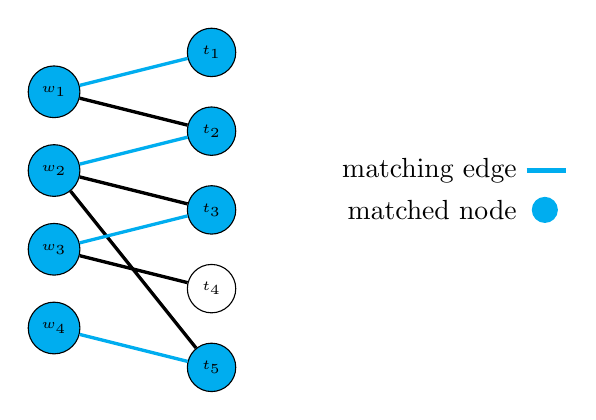
\begin{tikzpicture}
\node[draw, circle, fill=cyan] (w1) at (0, 3.5) {\tiny $w_1$};
\node[draw, circle, fill=cyan] (w2) at (0, 2.5) {\tiny $w_2$};
\node[draw, circle, fill=cyan] (w3) at (0, 1.5) {\tiny $w_3$};
\node[draw, circle, fill=cyan] (w4) at (0, 0.5) {\tiny $w_4$};

\node[draw, circle, fill=cyan] (t1) at (2, 4) {\tiny $t_1$};
\node[draw, circle, fill=cyan] (t2) at (2, 3) {\tiny $t_2$};
\node[draw, circle, fill=cyan] (t3) at (2, 2) {\tiny $t_3$};
\node[draw, circle] (t4) at (2, 1) {\tiny $t_4$};
\node[draw, circle, fill=cyan] (t5) at (2, 0) {\tiny $t_5$};

\draw[very thick, cyan] (w1) -- (t1);
\draw[very thick] (w1) -- (t2);
\draw[very thick, cyan] (w2) -- (t2);
\draw[very thick] (w2) -- (t3);
\draw[very thick] (w2) -- (t5);
\draw[very thick, cyan] (w3) -- (t3);
\draw[very thick] (w3) -- (t4);
\draw[very thick, cyan] (w4) -- (t5);

\def\x{6}
\def\y{3}
\draw (\x + 0, \y + -0.5) edge[color = cyan, line width=1.5pt] (\x + 0.5, \y + -0.5) node[text=black, anchor = east] {matching edge};
\node[anchor = east] (z) at (\x + 0, \y + -1) {matched node}; 
\node[circle, fill = cyan, right=0.06cm of z] {};

\end{tikzpicture}
\end{center}

We can see that, in this case, it is possible to assign every worker to some task as show in blue in the figure
(assign $w1$ to $t1$, $w2$ to $t2$, $w3$ to $t3$ and $w4$ to $t5$). \\

The set of blue edges is called a \emph{matching}. More generally, a matching is a subset of edges such that no
two edges share an endpoint. Because they share no endpoints, we know that each worker is assigned to at
most one task. \\

To compute such a solution, we start from an empty matching and try to iteratively increase its size.
In order to achieve this, we look for an \emph{augmenting path} in the graph. An augmenting path is a
path between two unmatched nodes that alternates between unmatched and matched edges. Before we continue,
let's take a look at the structure of an augmenting path.
\\

\begin{center}
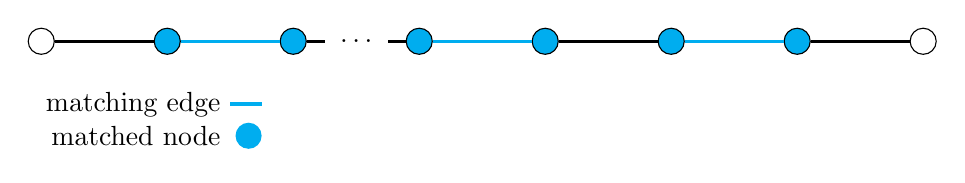
\begin{tikzpicture}[scale = 0.8]
\node[circle, draw] (x1) at (0, 0) {};
\node[circle, draw, fill=cyan] (x2) at (2, 0) {};
\node[circle, draw, fill=cyan] (x3) at (4, 0) {};
\node[circle, draw, fill=cyan] (x4) at (6, 0) {};
\node[circle, draw, fill=cyan] (x5) at (8, 0) {};
\node[circle, draw, fill=cyan] (x6) at (10, 0) {};
\node[circle, draw, fill=cyan] (x7) at (12, 0) {};
\node[circle, draw] (x8) at (14, 0) {};
%\draw[gray, opacity = 0.4, line width=6pt] (x1) -- (y1) -- (y2) -- (x6) -- (x7) -- (x8);
\draw[very thick] (x1) -- (x2);
\draw[very thick, cyan] (x2) -- (x3);
\draw[very thick] (x3) -- (4.5, 0);
\draw[very thick] (x4) -- (5.5, 0);
\node at (5, 0) {$\ldots$};
\draw[very thick, cyan] (x4) -- (x5);
\draw[very thick] (x5) -- (x6);
\draw[very thick, cyan] (x6) -- (x7);
\draw[very thick] (x7) -- (x8);

\def\x{3}
\def\y{-0.5}
\draw (\x + 0, \y + -0.5) edge[color = cyan, line width=1.5pt] (\x + 0.5, \y + -0.5) node[text=black, anchor = east] {matching edge};
\node[anchor = east] (z) at (\x + 0, \y + -1) {matched node}; 
\node[circle, fill = cyan, right=0.06cm of z] {};

\end{tikzpicture}
\end{center}

Any edge of the graph connecting a node from an augmenting path to a node
not in it must be an unmatched edge. The reason for this is that
every node except the first and the last are matched to another
node belonging to the path. Since a node cannot be matched to more
than one node, those nodes cannot have other matched edges
out of them. By definition, the first and the last nodes are unmatched so
they don't have matched edges going out of them. An augmenting path always has odd length. If it has a total
of $k$ matching edges, it will have $k + 1$ unmatched edges giving
a total of $2k + 1$ edges, which is odd. Finally, if we flip each edge
of an augmenting path (matched becomes unmatched and vice-versa),
the result is still a valid matching.

\begin{center}
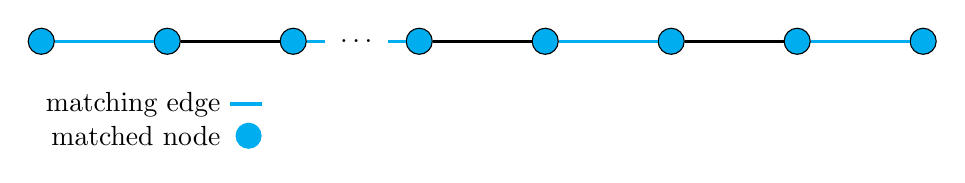
\begin{tikzpicture}[scale = 0.8]
\node[circle, draw, fill=cyan] (x1) at (0, 0) {};
\node[circle, draw, fill=cyan] (x2) at (2, 0) {};
\node[circle, draw, fill=cyan] (x3) at (4, 0) {};
\node[circle, draw, fill=cyan] (x4) at (6, 0) {};
\node[circle, draw, fill=cyan] (x5) at (8, 0) {};
\node[circle, draw, fill=cyan] (x6) at (10, 0) {};
\node[circle, draw, fill=cyan] (x7) at (12, 0) {};
\node[circle, draw, fill=cyan] (x8) at (14, 0) {};
%\draw[gray, opacity = 0.4, line width=6pt] (x1) -- (y1) -- (y2) -- (x6) -- (x7) -- (x8);
\draw[very thick, cyan] (x1) -- (x2);
\draw[very thick] (x2) -- (x3);
\draw[very thick, cyan] (x3) -- (4.5, 0);
\draw[very thick, cyan] (x4) -- (5.5, 0);
\node at (5, 0) {$\ldots$};
\draw[very thick] (x4) -- (x5);
\draw[very thick, cyan] (x5) -- (x6);
\draw[very thick] (x6) -- (x7);
\draw[very thick, cyan] (x7) -- (x8);

\def\x{3}
\def\y{-0.5}
\draw (\x + 0, \y + -0.5) edge[color = cyan, line width=1.5pt] (\x + 0.5, \y + -0.5) node[text=black, anchor = east] {matching edge};
\node[anchor = east] (z) at (\x + 0, \y + -1) {matched node}; 
\node[circle, fill = cyan, right=0.06cm of z] {};

\end{tikzpicture}
\end{center}

This is simply because, as we first observed, there are no matching
edges leaving an augmenting path. Hence there is no risk of having
some node in the path touching two matching edges after this. Moreover,
the size of the matching is increased because now we have $k + 1$
matching edges instead of $k$ in the path. \\

These properties will be
important later on so we summarize them:

\begin{itemize}
 \item there are no matching edges between a node in an augmenting path and a node outside that path;
 \item an augmenting path always has odd length;
 \item inverting each edge of the path yields a matching of size $+1$.
\end{itemize}

The basic algorithm to compute a maximum bipartite matching simply
consists on finding an augmenting path and reversing its edges while
such a path exists. \\
Let's try to understand why is it that a this algorithm works. On one hand,
it is clear that is some augmenting path exists, then by inverting the edges,
we get a bigger matching and therefore the initial matching could not be 
maximum. Now we need to understand why having no augmenting path makes a
matching optimal. One could think that maybe by finding some bad sequence
of augmenting paths we would reach a local maximum instead of a global
maximum. To prove that this is not the case, consider two matchings $M_1$ and $M_2$ such that $M_2$
is bigger than $M_1$. This obviously means that $M_1$ is not maximum. We are going
to show that using $M_2$ we can build an augmenting path for $M_1$. \\

Consider the subgraph formed by removing from
$G$ all edges that are in neither of the two matchings. This is a graph such that
each connected component is one of the following:

\begin{enumerate}
 \item a single node;
 \item a path alternating between $M_1$ and $M_2$;
 \item a cycle alternating between $M_1$ and $M_2$.
\end{enumerate}

For instance, the following figure shows two matchings on
a bipartite graph on the left and the subgraph obtained from
removing all edges that are unmatched. As we can see, the
connected components are indeed single nodes, alternating paths
and alternating cycles. Note that some edges might belong to both matchings like edge between
$e$ and $j$. \\


\begin{center}
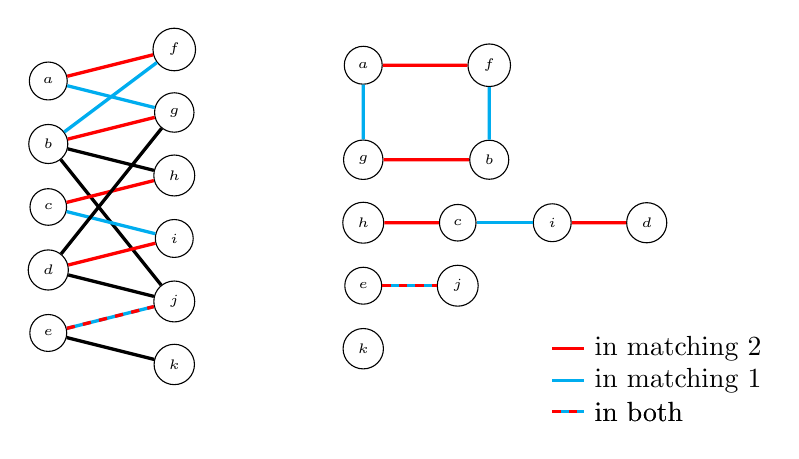
\begin{tikzpicture}[scale = 0.8]
\node[draw, circle] (a) at (0, 3.5) {\tiny $a$};
\node[draw, circle] (b) at (0, 2.5) {\tiny $b$};
\node[draw, circle] (c) at (0, 1.5) {\tiny $c$};
\node[draw, circle] (d) at (0, 0.5) {\tiny $d$};
\node[draw, circle] (e) at (0, -0.5) {\tiny $e$};

\node[draw, circle] (f) at (2, 4) {\tiny $f$};
\node[draw, circle] (g) at (2, 3) {\tiny $g$};
\node[draw, circle] (h) at (2, 2) {\tiny $h$};
\node[draw, circle] (i) at (2, 1) {\tiny $i$};
\node[draw, circle] (j) at (2, 0) {\tiny $j$};
\node[draw, circle] (k) at (2, -1) {\tiny $k$};


\draw[very thick, red] (a) -- (f);
\draw[very thick, cyan] (a) -- (g);
\draw[very thick, cyan] (b) -- (f);
\draw[very thick, red] (b) -- (g);
\draw[very thick] (b) -- (h);
\draw[very thick] (b) -- (j);
\draw[very thick, red] (c) -- (h);
\draw[very thick, cyan] (c) -- (i);
\draw[very thick] (d) -- (g);
\draw[very thick, red] (d) -- (i);
\draw[very thick] (d) -- (j);
\draw[very thick, cyan] (e) -- (j);
\draw[very thick, dashed, red] (e) -- (j);
\draw[very thick] (e) -- (k);


\node[draw, circle] (A) at (5, 3.75) {\tiny $a$};
\node[draw, circle] (F) at (7, 3.75) {\tiny $f$};
\node[draw, circle] (G) at (5, 2.25) {\tiny $g$};
\node[draw, circle] (B) at (7, 2.25) {\tiny $b$};

\draw[very thick, red] (A) -- (F);
\draw[very thick, red] (G) -- (B);
\draw[very thick, cyan] (A) -- (G);
\draw[very thick, cyan] (B) -- (F);

\node[draw, circle] (H) at (5, 1.25) {\tiny $h$};
\node[draw, circle] (C) at (6.5, 1.25) {\tiny $c$};
\node[draw, circle] (I) at (8, 1.25) {\tiny $i$};
\node[draw, circle] (D) at (9.5, 1.25) {\tiny $d$};

\draw[very thick, red] (H) -- (C);
\draw[very thick, cyan] (C) -- (I);
\draw[very thick, red] (I) -- (D);


\node[draw, circle] (E) at (5, 0.25) {\tiny $e$};
\node[draw, circle] (J) at (6.5, 0.25) {\tiny $j$};

\node[draw, circle] (K) at (5, -0.75) {\tiny $k$};

\draw[very thick, cyan] (E) -- (J);
\draw[very thick, red, dashed] (E) -- (J);


\draw[very thick, red] (8, -0.75) -- (8.5, -0.75) node[color = black, anchor = west] {in matching 2};
\draw[very thick, cyan] (8, -1.25) -- (8.5, -1.25) node[color = black, anchor = west] {in matching 1};
\draw[very thick, cyan] (8, -1.75) -- (8.5, -1.75) node[color = black, anchor = west] {in both};
\draw[very thick, red, dashed] (8, -1.75) -- (8.5, -1.75) node[color = black, anchor = west] {in both};

\end{tikzpicture}
\end{center}


The reason why this is true in general is that each matching
forms a subgraph where each node has either degree $0$ or $1$. When we combine
both there graphs we get a graph where each node has either degree $0$, $1$
or $2$. Such a graph can only be a collection of isolated nodes, paths
and cycles. These paths (and cycles) must alternate between $M_1$ and $M_2$ is because,
being matchings, no node can be connected to two edges of the same matching. \\

Now, the cycles must be composed of an even number of edges. Half from
the first matching and the other half from the second. If it was odd, we would have one node connected
by two edges of the same matching which violates the matching definition. Therefore, since
$M_2$ is bigger than $M_1$, there must be some component that is a path
and that contains more edges from $M_2$ than $M_1$. That path must be
an alternating path on the graph with respect to $M_1$ (this path is $(h, c, i, d)$ in
the example). \\

This result is known as \emph{Berge's lemma}. \\

All this justifies that given a matching $M$ on a graph $G$ (not necessarily bipartite as we did not use
the bipartiteness of $G$ in our argument), $M$
is maximum if and only if there is no augmenting path on $G$ with respect to $M$. Thus the algorithm
to compute a maximum matching in general simply consists on starting from an empty matching, successively
finding augmenting paths and increasing the current matching by reversing the edges from the path.

\begin{enumerate}
 \item $M = \emptyset$
 \item while $G$ contains an augmenting path with respect to $M$
\begin{enumerate}
 \item find an augmenting path $p$ with respect to $M$
 \item increase $M$ by reversing the edges of $p$
\end{enumerate} 
\end{enumerate}

Therefore we have reduced the problem of computing a maximum matching to the problem of computing augmenting paths.
The next figure shows an illustration of the execution of the algorithm on a bipartite
graph.

%\setlength{\tabcolsep}{10pt}

\begin{center}
\begin{tabular}{c c c c}
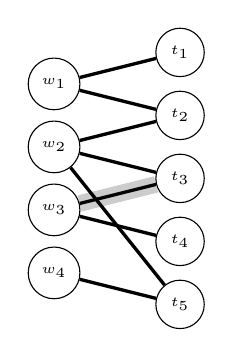
\begin{tikzpicture}[scale = 0.8]
\node[draw, circle] (w1) at (0, 3.5) {\tiny $w_1$};
\node[draw, circle] (w2) at (0, 2.5) {\tiny $w_2$};
\node[draw, circle] (w3) at (0, 1.5) {\tiny $w_3$};
\node[draw, circle] (w4) at (0, 0.5) {\tiny $w_4$};

\node[draw, circle] (t1) at (2, 4) {\tiny $t_1$};
\node[draw, circle] (t2) at (2, 3) {\tiny $t_2$};
\node[draw, circle] (t3) at (2, 2) {\tiny $t_3$};
\node[draw, circle] (t4) at (2, 1) {\tiny $t_4$};
\node[draw, circle] (t5) at (2, 0) {\tiny $t_5$};


\draw[gray, opacity = 0.4, line width=6pt] (w3) -- (t3);

\draw[very thick] (w1) -- (t1);
\draw[very thick] (w1) -- (t2);
\draw[very thick] (w2) -- (t2);
\draw[very thick] (w2) -- (t3);
\draw[very thick] (w2) -- (t5);
\draw[very thick] (w3) -- (t3);
\draw[very thick] (w3) -- (t4);
\draw[very thick] (w4) -- (t5);
\end{tikzpicture}
&
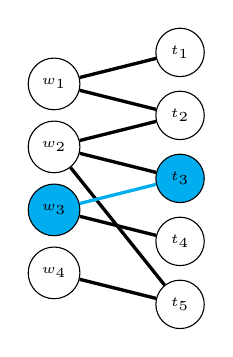
\begin{tikzpicture}[scale = 0.8]
\node[draw, circle] (w1) at (0, 3.5) {\tiny $w_1$};
\node[draw, circle] (w2) at (0, 2.5) {\tiny $w_2$};
\node[draw, circle, fill=cyan] (w3) at (0, 1.5) {\tiny $w_3$};
\node[draw, circle] (w4) at (0, 0.5) {\tiny $w_4$};

\node[draw, circle] (t1) at (2, 4) {\tiny $t_1$};
\node[draw, circle] (t2) at (2, 3) {\tiny $t_2$};
\node[draw, circle, fill=cyan] (t3) at (2, 2) {\tiny $t_3$};
\node[draw, circle] (t4) at (2, 1) {\tiny $t_4$};
\node[draw, circle] (t5) at (2, 0) {\tiny $t_5$};

\draw[very thick] (w1) -- (t1);
\draw[very thick] (w1) -- (t2);
\draw[very thick] (w2) -- (t2);
\draw[very thick] (w2) -- (t3);
\draw[very thick] (w2) -- (t5);
\draw[very thick, cyan] (w3) -- (t3);
\draw[very thick] (w3) -- (t4);
\draw[very thick] (w4) -- (t5);
\end{tikzpicture}
&
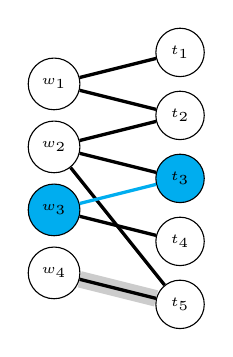
\begin{tikzpicture}[scale = 0.8]
\node[draw, circle] (w1) at (0, 3.5) {\tiny $w_1$};
\node[draw, circle] (w2) at (0, 2.5) {\tiny $w_2$};
\node[draw, circle, fill=cyan] (w3) at (0, 1.5) {\tiny $w_3$};
\node[draw, circle] (w4) at (0, 0.5) {\tiny $w_4$};

\node[draw, circle] (t1) at (2, 4) {\tiny $t_1$};
\node[draw, circle] (t2) at (2, 3) {\tiny $t_2$};
\node[draw, circle, fill=cyan] (t3) at (2, 2) {\tiny $t_3$};
\node[draw, circle] (t4) at (2, 1) {\tiny $t_4$};
\node[draw, circle] (t5) at (2, 0) {\tiny $t_5$};
\draw[gray, opacity = 0.4, line width=6pt] (w4) -- (t5);
\draw[very thick] (w1) -- (t1);
\draw[very thick] (w1) -- (t2);
\draw[very thick] (w2) -- (t2);
\draw[very thick] (w2) -- (t3);
\draw[very thick] (w2) -- (t5);
\draw[very thick, cyan] (w3) -- (t3);
\draw[very thick] (w3) -- (t4);
\draw[very thick] (w4) -- (t5);

\end{tikzpicture}
&
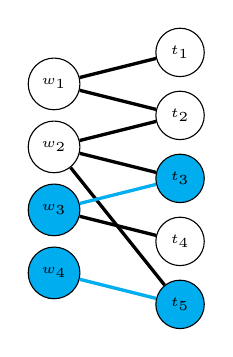
\begin{tikzpicture}[scale = 0.8]
\node[draw, circle] (w1) at (0, 3.5) {\tiny $w_1$};
\node[draw, circle] (w2) at (0, 2.5) {\tiny $w_2$};
\node[draw, circle, fill=cyan] (w3) at (0, 1.5) {\tiny $w_3$};
\node[draw, circle, fill=cyan] (w4) at (0, 0.5) {\tiny $w_4$};

\node[draw, circle] (t1) at (2, 4) {\tiny $t_1$};
\node[draw, circle] (t2) at (2, 3) {\tiny $t_2$};
\node[draw, circle, fill=cyan] (t3) at (2, 2) {\tiny $t_3$};
\node[draw, circle] (t4) at (2, 1) {\tiny $t_4$};
\node[draw, circle, fill=cyan] (t5) at (2, 0) {\tiny $t_5$};
\draw[very thick] (w1) -- (t1);
\draw[very thick] (w1) -- (t2);
\draw[very thick] (w2) -- (t2);
\draw[very thick] (w2) -- (t3);
\draw[very thick] (w2) -- (t5);
\draw[very thick, cyan] (w3) -- (t3);
\draw[very thick] (w3) -- (t4);
\draw[very thick, cyan] (w4) -- (t5);

\end{tikzpicture}

\\[0.2cm]

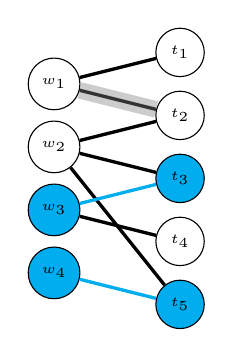
\begin{tikzpicture}[scale = 0.8]
\node[draw, circle] (w1) at (0, 3.5) {\tiny $w_1$};
\node[draw, circle] (w2) at (0, 2.5) {\tiny $w_2$};
\node[draw, circle, fill=cyan] (w3) at (0, 1.5) {\tiny $w_3$};
\node[draw, circle, fill=cyan] (w4) at (0, 0.5) {\tiny $w_4$};

\node[draw, circle] (t1) at (2, 4) {\tiny $t_1$};
\node[draw, circle] (t2) at (2, 3) {\tiny $t_2$};
\node[draw, circle, fill=cyan] (t3) at (2, 2) {\tiny $t_3$};
\node[draw, circle] (t4) at (2, 1) {\tiny $t_4$};
\node[draw, circle, fill=cyan] (t5) at (2, 0) {\tiny $t_5$};
\draw[very thick] (w1) -- (t1);
\draw[very thick] (w1) -- (t2);
\draw[very thick] (w2) -- (t2);
\draw[very thick] (w2) -- (t3);
\draw[very thick] (w2) -- (t5);
\draw[very thick, cyan] (w3) -- (t3);
\draw[very thick] (w3) -- (t4);
\draw[very thick, cyan] (w4) -- (t5);
\draw[gray, opacity = 0.4, line width=6pt] (w1) -- (t2);
\end{tikzpicture}

&

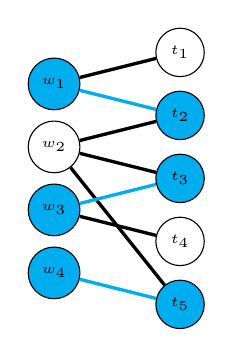
\begin{tikzpicture}[scale = 0.8]
\node[draw, circle, fill=cyan] (w1) at (0, 3.5) {\tiny $w_1$};
\node[draw, circle] (w2) at (0, 2.5) {\tiny $w_2$};
\node[draw, circle, fill=cyan] (w3) at (0, 1.5) {\tiny $w_3$};
\node[draw, circle, fill=cyan] (w4) at (0, 0.5) {\tiny $w_4$};

\node[draw, circle] (t1) at (2, 4) {\tiny $t_1$};
\node[draw, circle, fill=cyan] (t2) at (2, 3) {\tiny $t_2$};
\node[draw, circle, fill=cyan] (t3) at (2, 2) {\tiny $t_3$};
\node[draw, circle] (t4) at (2, 1) {\tiny $t_4$};
\node[draw, circle, fill=cyan] (t5) at (2, 0) {\tiny $t_5$};
\draw[very thick] (w1) -- (t1);
\draw[very thick, cyan] (w1) -- (t2);
\draw[very thick] (w2) -- (t2);
\draw[very thick] (w2) -- (t3);
\draw[very thick] (w2) -- (t5);
\draw[very thick, cyan] (w3) -- (t3);
\draw[very thick] (w3) -- (t4);
\draw[very thick, cyan] (w4) -- (t5);
\end{tikzpicture}

&

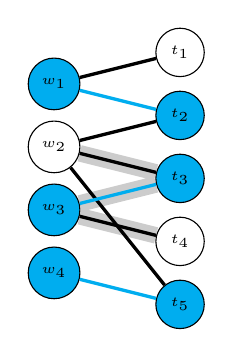
\begin{tikzpicture}[scale = 0.8]
\node[draw, circle, fill=cyan] (w1) at (0, 3.5) {\tiny $w_1$};
\node[draw, circle] (w2) at (0, 2.5) {\tiny $w_2$};
\node[draw, circle, fill=cyan] (w3) at (0, 1.5) {\tiny $w_3$};
\node[draw, circle, fill=cyan] (w4) at (0, 0.5) {\tiny $w_4$};

\node[draw, circle] (t1) at (2, 4) {\tiny $t_1$};
\node[draw, circle, fill=cyan] (t2) at (2, 3) {\tiny $t_2$};
\node[draw, circle, fill=cyan] (t3) at (2, 2) {\tiny $t_3$};
\node[draw, circle] (t4) at (2, 1) {\tiny $t_4$};
\node[draw, circle, fill=cyan] (t5) at (2, 0) {\tiny $t_5$};
\draw[gray, opacity = 0.4, line width=6pt] (t4) -- (w3) -- (t3) -- (w2);
\draw[very thick] (w1) -- (t1);
\draw[very thick, cyan] (w1) -- (t2);
\draw[very thick] (w2) -- (t2);
\draw[very thick] (w2) -- (t3);
\draw[very thick] (w2) -- (t5);
\draw[very thick, cyan] (w3) -- (t3);
\draw[very thick] (w3) -- (t4);
\draw[very thick, cyan] (w4) -- (t5);
\end{tikzpicture}

&

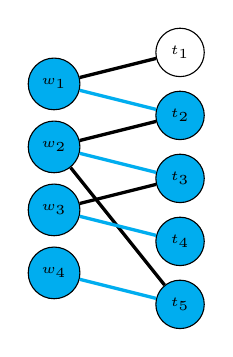
\begin{tikzpicture}[scale = 0.8]
\node[draw, circle, fill=cyan] (w1) at (0, 3.5) {\tiny $w_1$};
\node[draw, circle, fill=cyan] (w2) at (0, 2.5) {\tiny $w_2$};
\node[draw, circle, fill=cyan] (w3) at (0, 1.5) {\tiny $w_3$};
\node[draw, circle, fill=cyan] (w4) at (0, 0.5) {\tiny $w_4$};

\node[draw, circle] (t1) at (2, 4) {\tiny $t_1$};
\node[draw, circle, fill=cyan] (t2) at (2, 3) {\tiny $t_2$};
\node[draw, circle, fill=cyan] (t3) at (2, 2) {\tiny $t_3$};
\node[draw, circle, fill=cyan] (t4) at (2, 1) {\tiny $t_4$};
\node[draw, circle, fill=cyan] (t5) at (2, 0) {\tiny $t_5$};
\draw[very thick] (w1) -- (t1);
\draw[very thick, cyan] (w1) -- (t2);
\draw[very thick] (w2) -- (t2);
\draw[very thick, cyan] (w2) -- (t3);
\draw[very thick] (w2) -- (t5);
\draw[very thick] (w3) -- (t3);
\draw[very thick, cyan] (w3) -- (t4);
\draw[very thick, cyan] (w4) -- (t5);
\end{tikzpicture}

\\


&

&

&

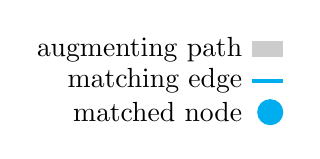
\begin{tikzpicture}[scale = 0.8]
\draw (0, 0) edge[color = gray, opacity = 0.4, line width=6pt] (0.5, 0) node[text=black, anchor = east] {augmenting path};
\draw (0, -0.5) edge[color = cyan, line width=1.5pt] (0.5, -0.5) node[text=black, anchor = east] {matching edge};
\node[anchor = east] (z) at (0, -1) {matched node}; 
\node[circle, fill = cyan, right=0.06cm of z] {};
\end{tikzpicture}


\end{tabular}
\end{center}

The problem of finding an augmenting path may seem easy at first sight but it is actually quite tricky.
If you try to find such a path with \textsf{BFS} or \textsf{DFS} you will fail to find to find
some paths. To see this, consider the following graph. There is only one augmenting path 
$(c, e, f, d, b, a)$. If you start your \textsf{BFS} from $c$, at the first iteration $b$ will be
marked as visited. Therefore when you arrive from $d$ you will not visit it and you will
fail to find the path. If you start from $a$, node $d$ will mark both $e$ and $f$ as visited
and thus $f$ will fail to visit $e$. The same happens with a DFS if the nodes are expanded
in alphabetical order. Note that for the \textsf{DFS}, there always exists an ordering of the 
adjacent nodes that makes it so that \textsf{DFS} finds the augmenting path if one exists. But there is
no guarantee that the nodes will be given in that order and it is easy to make 
instances where the probability of finding that order is as small as we want.

\begin{center}
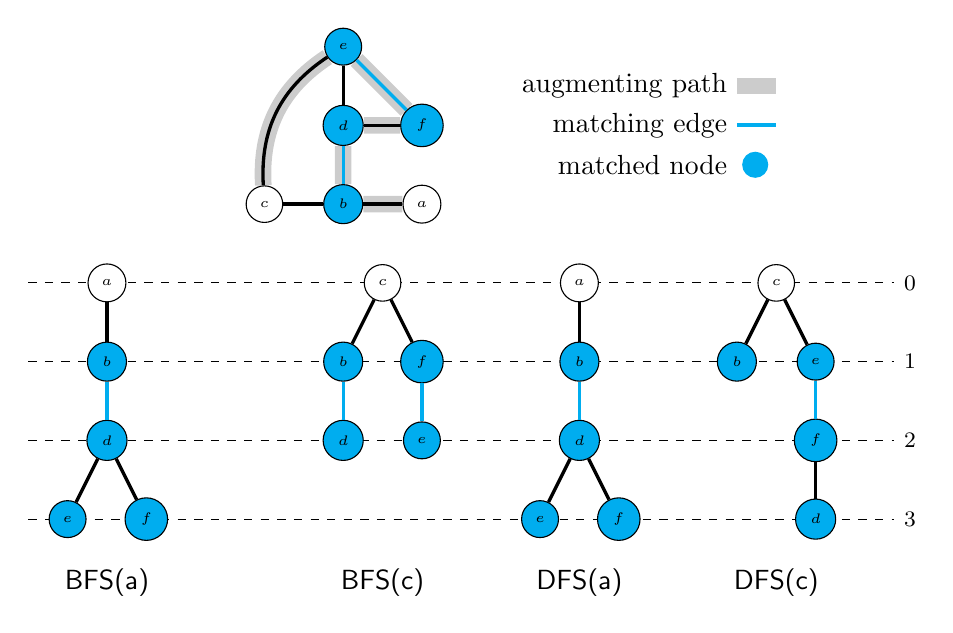
\begin{tikzpicture}

\def\x{3}
\def\y{0}

\node[draw, circle] (a) at (\x + 0, \y + 0) {\tiny $a$};
\node[draw, circle, fill=cyan] (b) at (\x + -1, \y + 0) {\tiny $b$};
\node[draw, circle] (c) at (\x + -2, \y + 0) {\tiny $c$};
\node[draw, circle, fill=cyan] (d) at (\x + -1, \y + 1) {\tiny $d$};
\node[draw, circle, fill=cyan] (e) at (\x + 0, \y + 1) {\tiny $f$};
\node[draw, circle, fill=cyan] (f) at (\x + -1, \y + 2) {\tiny $e$};

\draw[gray, opacity = 0.4, line width=6pt] (a) -- (b) -- (d) -- (e) -- (f);
\draw (f) edge[gray, opacity = 0.4, line width=6pt, bend right] (c);

\draw[very thick] (a) -- (b);
\draw[very thick] (b) -- (c);
\draw[very thick, cyan] (b) -- (d);
\draw[very thick] (d) -- (e);
\draw[very thick, cyan] (e) -- (f);
\draw[very thick] (d) -- (f);
\draw[very thick] (c) edge[bend left] (f);

\def\x{7}
\def\y{1.5}
\draw (\x + 0, \y + 0) edge[color = gray, opacity = 0.4, line width=6pt] (\x + 0.5, \y + 0) node[text=black, anchor = east] {augmenting path};
\draw (\x + 0, \y + -0.5) edge[color = cyan, line width=1.5pt] (\x + 0.5, \y + -0.5) node[text=black, anchor = east] {matching edge};
\node[anchor = east] (z) at (\x + 0, \y + -1) {matched node}; 
\node[circle, fill = cyan, right=0.06cm of z] {};

\def\x{-1}
\def\y{-1}

\draw[dashed] (\x + -1, \y + 0) -- (\x + 10, \y + 0) node[anchor=west] {\footnotesize 0};
\draw[dashed] (\x + -1, \y + -1) -- (\x + 10, \y + -1) node[anchor=west] {\footnotesize 1};
\draw[dashed] (\x + -1, \y + -2) -- (\x + 10, \y + -2) node[anchor=west] {\footnotesize 2};
\draw[dashed] (\x + -1, \y + -3) -- (\x + 10, \y + -3) node[anchor=west] {\footnotesize 3};


\node[draw, circle, fill=white] (a) at (0 + \x, \y + 0) {\tiny $a$};
\node[draw, circle, fill=cyan] (b) at (0 + \x, \y + -1) {\tiny $b$};
\node[draw, circle, fill=cyan] (d) at (0 + \x,  \y + -2) {\tiny $d$};
\node[draw, circle, fill=cyan] (e) at (-0.5 + \x, \y + -3) {\tiny $e$};
\node[draw, circle, fill=cyan] (f) at (0.5 + \x, \y + -3) {\tiny $f$};

\draw[very thick] (a) -- (b);
\draw[very thick, cyan] (b) -- (d);
\draw[very thick] (d) -- (e);
\draw[very thick] (d) -- (f);

\node at (\x + 0, -4.8) {\textsf{BFS(a)}};

\def\x{2.5}

\node[draw, circle, fill=white] (c) at (0 + \x, \y + 0) {\tiny $c$};
\node[draw, circle, fill=cyan] (b) at (-0.5 + \x, \y + -1) {\tiny $b$};
\node[draw, circle, fill=cyan] (f) at (0.5 + \x, \y + -1) {\tiny $f$};

\node[draw, circle, fill=cyan] (d) at (-0.5 + \x, \y + -2) {\tiny $d$};
\node[draw, circle, fill=cyan] (e) at (0.5 + \x, \y + -2) {\tiny $e$};


\draw[very thick] (c) -- (b);
\draw[very thick] (c) -- (f);
\draw[very thick, cyan] (b) -- (d);
\draw[very thick, cyan] (f) -- (e);

\node at (\x + 0, -4.8) {\textsf{BFS(c)}};

\def\x{5}

\node[draw, circle, fill=white] (a) at (0 + \x, \y + 0) {\tiny $a$};
\node[draw, circle, fill=white, fill=cyan] (b) at (0 + \x, \y + -1) {\tiny $b$};
\node[draw, circle, fill=white, fill=cyan] (d) at (0 + \x, \y + -2) {\tiny $d$};
\node[draw, circle, fill=white, fill=cyan] (e) at (-0.5 + \x, \y + -3) {\tiny $e$};
\node[draw, circle, fill=white, fill=cyan] (f) at (0.5 + \x, \y + -3) {\tiny $f$};

\draw[very thick] (a) -- (b);
\draw[very thick, cyan] (b) -- (d);
\draw[very thick] (d) -- (e);
\draw[very thick] (d) -- (f);

\node at (\x + 0, -4.8) {\textsf{DFS(a)}};

\def\x{7.5}

\node[draw, circle, fill=white] (c) at (0 + \x, \y + 0) {\tiny $c$};
\node[draw, circle, fill=cyan] (b) at (-0.5 + \x, \y + -1) {\tiny $b$};
\node[draw, circle, fill=cyan] (e) at (0.5 + \x, \y + -1) {\tiny $e$};
\node[draw, circle, fill=cyan] (f) at (0.5 + \x, \y + -2) {\tiny $f$};
\node[draw, circle, fill=cyan] (d) at (0.5 + \x, \y + -3) {\tiny $d$};

\draw[very thick] (c) -- (b);
\draw[very thick] (c) -- (e);
\draw[very thick, cyan] (e) -- (f);
\draw[very thick] (f) -- (d);

\node at (\x + 0, -4.8) {\textsf{DFS(c)}};

\end{tikzpicture}
\end{center}

The next idea that comes to mind after this is to allow to visit the nodes twice,
one time coming from a matched edge and another time coming from an unmatched edge. This
also does not work but for a different reason. In this case it can happen that the algorithm
says that a path exists when actually no such path exists. This is because the 
output of the algorithm may contain cycles. The following graph shows an example.

\begin{center}
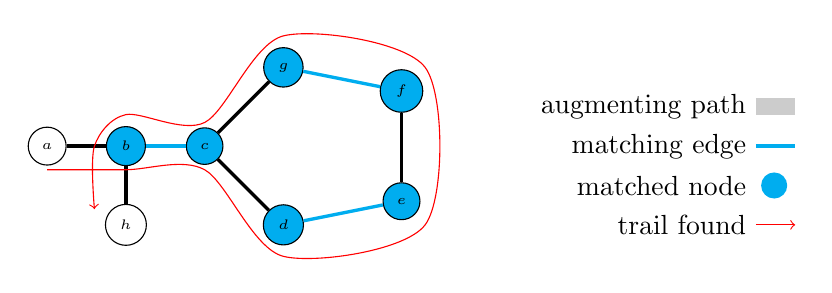
\begin{tikzpicture}
\def\x{0}
\def\y{0}
\node[draw, circle] (a) at (\x + 0, \y + 0) {\tiny $a$};
\node[draw, circle, fill=cyan] (b) at (\x + 1, \y + 0) {\tiny $b$};
\node[draw, circle, fill=cyan] (c) at (\x + 2, \y + 0) {\tiny $c$};
\node[draw, circle, fill=cyan] (d) at (\x + 3, \y - 1) {\tiny $d$};
\node[draw, circle, fill=cyan] (e) at (\x + 4.5, \y - 0.7) {\tiny $e$};
\node[draw, circle, fill=cyan] (f) at (\x + 4.5, \y + 0.7) {\tiny $f$};
\node[draw, circle, fill=cyan] (g) at (\x + 3, \y + 1) {\tiny $g$};
\node[draw, circle] (h) at (\x + 1, \y - 1) {\tiny $h$};


\draw[very thick] (a) -- (b);
\draw[very thick, cyan] (b) -- (c);
\draw[very thick] (c) -- (d);
\draw[very thick, cyan] (d) -- (e);
\draw[very thick] (e) -- (f);
\draw[very thick, cyan] (f) -- (g);
\draw[very thick] (g) -- (c);
\draw[very thick] (b) -- (h);

\draw [red, ->] plot [smooth] coordinates {(0,-0.3) (1, -0.3) (2, -0.3) (3, -1.4) (4.8, -1) (4.8, 1) (3, 1.4) (2, 0.3) (1, 0.4) (0.6, 0) (0.6, -0.8)};

\def\x{9}
\def\y{0.5}
\draw (\x + 0, \y + 0) edge[color = gray, opacity = 0.4, line width=6pt] (\x + 0.5, \y + 0) node[text=black, anchor = east] {augmenting path};
\draw (\x + 0, \y + -0.5) edge[color = cyan, line width=1.5pt] (\x + 0.5, \y + -0.5) node[text=black, anchor = east] {matching edge};
\node[anchor = east] (z) at (\x + 0, \y + -1) {matched node}; 
\node[circle, fill = cyan, right=0.06cm of z] {};
\draw (\x + 0, \y + -1.5) edge[color = red, ->] (\x + 0.5, \y + -1.5) node[text=black, anchor = east] {trail found};

\end{tikzpicture}
\end{center}

The double label algorithm will find the trail shown in red which is not valid since it
visits nodes $b$ and $c$ twice. The reason is that when it arrives at $c$ from $g$, $c$
was never visited while arriving via an unmatched edge. So to the algorithm proceeds. The same
happens at $b$, which was never visited yet via an matched edge. \\

However we know that a simple \textsf{BFS} and \textsf{DFS} works for bipartite graphs. And we know that 
a graph is bipartite if and only if it contains no odd cycles. So what is it about 
odd cycles that make the algorithms fail? Actually it is not so much odd cycles but
\emph{odd alternating cycles}. An odd alternating cycle is a cycle 
$(x_1, x_2, x_3, \ldots, x_{2k + 1})$ such that:

\begin{enumerate}
 \item $(x_1, x_2)$ and $(x_1, x_{2k + 1})$ are unmatched;
 \item edges in the cycle alternate between unmatched and matched.
\end{enumerate}

It is not hard to see that a graph contains an alternating odd cycle with
respect to some matching $M$ reachable from an
unmatched node $x$ if and only if and only if there exists a node $y$
such that there exist two alternating paths from $x$ to $y$ one of them
ending with a matched edge and the other ending with an unmatched edge. \\

Clearly is such a cycle exists then $(x_1, x_{2k + 1})$ and
$(x_1, x_2, \ldots, x_{2k + 1})$ are two such paths (with $x = x_1$ and $y = x_{k +1})$. 
See the next figure for $k = 2$ for clarity.

\begin{center}
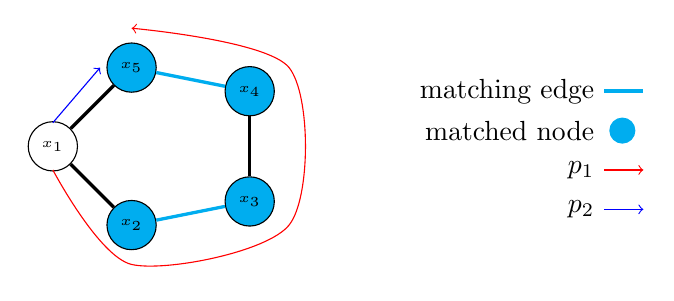
\begin{tikzpicture}
\node[draw, circle] (a) at (0, 0) {\tiny $x_1$};
\node[draw, circle, fill=cyan] (b) at (1, -1) {\tiny $x_2$};
\node[draw, circle, fill=cyan] (c) at (2.5, -0.7) {\tiny $x_3$};
\node[draw, circle, fill=cyan] (d) at (2.5, 0.7) {\tiny $x_4$};
\node[draw, circle, fill=cyan] (e) at (1, 1) {\tiny $x_5$};

\draw[very thick] (a) -- (b);
\draw[very thick, cyan] (b) -- (c);
\draw[very thick] (c) -- (d);
\draw[very thick, cyan] (d) -- (e);
\draw[very thick] (e) -- (a);

\draw [red, ->] plot [smooth] coordinates {(0,-0.3) (1, -1.5) (3, -1) (3, 1) (1, 1.5)};
\draw [blue, ->] plot [smooth] coordinates {(0,0.3) (0.6, 1)};

\def\x{7}
\def\y{1.2}
\draw (\x + 0, \y + -0.5) edge[color = cyan, line width=1.5pt] (\x + 0.5, \y + -0.5) node[text=black, anchor = east] {matching edge};
\node[anchor = east] (z) at (\x + 0, \y + -1) {matched node}; 
\node[circle, fill = cyan, right=0.06cm of z] {};
\draw (\x + 0, \y + -1.5) edge[color = red, ->] (\x + 0.5, \y + -1.5) node[text=black, anchor = east] {$p_1$};
\draw (\x + 0, \y + -2) edge[color = blue, ->] (\x + 0.5, \y + -2) node[text=black, anchor = east] {$p_2$};

\end{tikzpicture}
\end{center}

Now, suppose on the other hand that such paths exist, call them $p_1$, $p_2$.
These paths must meet at some node $z$ (maybe $z = x$). Since
the paths are alternating, there cannot be a matching edge between them (we saw
above that no matching edge can exit an alternating path). Hence both paths
will connect via an unmatched edge. Furthermore, the edge of $p_1$
ending in $z$ when walking from $x$ must be a matching edge otherwise
$p_2$ would not be alternating as the following picture shows
(we have two unmatched edges in a row).

\begin{center}
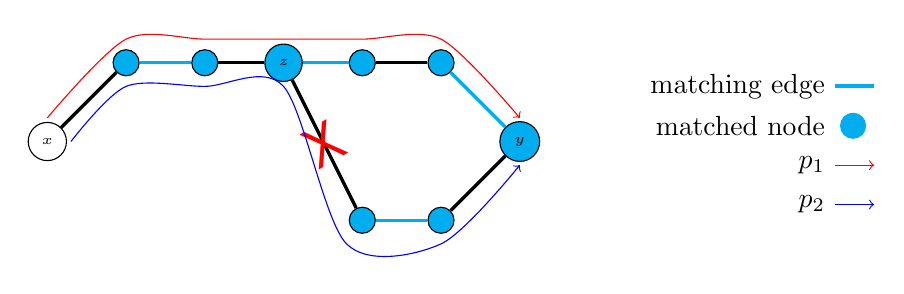
\begin{tikzpicture}

\node[draw, circle, fill=cyan] (y) at (5, 0) {\tiny $y$};
\node[draw, circle, fill=cyan] (b) at (4, 1) {};
\node[draw, circle, fill=cyan] (c) at (4, -1) {};
\node[draw, circle, fill=cyan] (d) at (3, 1) {};
\node[draw, circle, fill=cyan] (e) at (2, 1) {\tiny $z$};
\node[draw, circle, fill=cyan] (g) at (1, 1) {};
\node[draw, circle, fill=cyan] (h) at (0, 1) {};
\node[draw, circle, fill=cyan] (i) at (3, -1) {};

\node[draw, circle] (x) at (-1, 0) {\tiny $x$};

\draw[very thick, cyan] (y) -- (b);
\draw[very thick] (y) -- (c);
\draw[very thick] (b) -- (d);
\draw[very thick, cyan] (d) -- (e);
\draw[very thick] (e) -- (g);
\draw[very thick, cyan] (g) -- (h);
\draw[very thick] (x) -- (h);
\draw[very thick, cyan] (c) -- (i);

\draw[very thick] (i) edge node[red, rotate = 30] {\huge \textsf{X}} (e);

\draw [red, ->] plot [smooth] coordinates {(-1,0.3) (0, 1.3) (1, 1.3) (2, 1.3) (3, 1.3) (4, 1.3) (5, 0.3)};
\draw [blue, ->] plot [smooth] coordinates {(-0.7,0) (0, 0.7) (1, 0.7) (2, 0.7) (2.8, -1.3) (4, -1.3) (5, -0.3)};


\def\x{9}
\def\y{1.2}
\draw (\x + 0, \y + -0.5) edge[color = cyan, line width=1.5pt] (\x + 0.5, \y + -0.5) node[text=black, anchor = east] {matching edge};
\node[anchor = east] (z) at (\x + 0, \y + -1) {matched node}; 
\node[circle, fill = cyan, right=0.06cm of z] {};
\draw (\x + 0, \y + -1.5) edge[color = red, ->] (\x + 0.5, \y + -1.5) node[text=black, anchor = east] {$p_1$};
\draw (\x + 0, \y + -2) edge[color = blue, ->] (\x + 0.5, \y + -2) node[text=black, anchor = east] {$p_2$};

\end{tikzpicture}
\end{center}

This means that we have situation shown in the next figure. As we can see, this
gives an odd alternating cycle. The fact that the cycle has odd length comes from
the fact that the sub-path of $p_1$ form $z$ to $y$ starts with an unmatched edge
and ends with a matching edge. Hence it must have even length (same number of
matching and unmatched edges). On the other hand
the sub-path of $p_2$ from $z$ to $y$ starts with an unmatched edge and ends
with an unmatched edge. Thus it must have odd length (one more unmatched edge
than matching edges). \\

The hypothesis that $x$ is unmatched is important because it guarantees that
if $z = x$ then it still holds both paths exit $z$ with unmatched edges. This
is necessary in the definition of odd alternating cycle.

\begin{center}
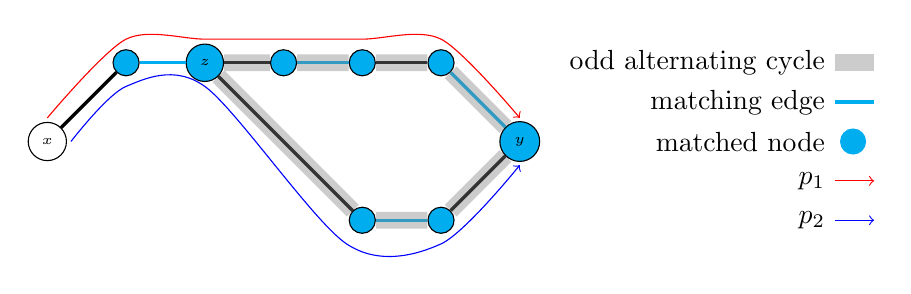
\begin{tikzpicture}

\node[draw, circle, fill=cyan] (y) at (5, 0) {\tiny $y$};
\node[draw, circle, fill=cyan] (b) at (4, 1) {};
\node[draw, circle, fill=cyan] (c) at (4, -1) {};
\node[draw, circle, fill=cyan] (d) at (3, 1) {};
\node[draw, circle, fill=cyan] (e) at (2, 1) {};
\node[draw, circle, fill=cyan] (g) at (1, 1) {\tiny $z$};
\node[draw, circle, fill=cyan] (h) at (0, 1) {};
\node[draw, circle, fill=cyan] (i) at (3, -1) {};

\node[draw, circle] (x) at (-1, 0) {\tiny $x$};

\draw[very thick, cyan] (y) -- (b);
\draw[very thick] (y) -- (c);
\draw[very thick] (b) -- (d);
\draw[very thick, cyan] (d) -- (e);
\draw[very thick] (e) -- (g);
\draw[very thick, cyan] (g) -- (h);
\draw[very thick] (x) -- (h);
\draw[very thick, cyan] (c) -- (i);

\draw[very thick] (i) -- (g);

\draw [red, ->] plot [smooth] coordinates {(-1,0.3) (0, 1.3) (1, 1.3) (2, 1.3) (3, 1.3) (4, 1.3) (5, 0.3)};
\draw [blue, ->] plot [smooth] coordinates {(-0.7,0) (0, 0.7) (1, 0.7) (2.8, -1.3) (4, -1.3) (5, -0.3)};

\draw[gray, opacity = 0.4, line width=6pt] (g) -- (e) -- (d) -- (b) -- (y) -- (c) -- (i) -- (g);


\def\x{9}
\def\y{1}
\draw (\x + 0, \y + -0.5) edge[color = cyan, line width=1.5pt] (\x + 0.5, \y + -0.5) node[text=black, anchor = east] {matching edge};
\node[anchor = east] (z) at (\x + 0, \y + -1) {matched node}; 
\node[circle, fill = cyan, right=0.06cm of z] {};
\draw (\x + 0, \y + -1.5) edge[color = red, ->] (\x + 0.5, \y + -1.5) node[text=black, anchor = east] {$p_1$};
\draw (\x + 0, \y + -2) edge[color = blue, ->] (\x + 0.5, \y + -2) node[text=black, anchor = east] {$p_2$};
\draw (\x + 0, \y + 0) edge[color = gray, opacity = 0.4, line width=6pt] (\x + 0.5, \y + 0) node[text=black, anchor = east] {odd alternating cycle};

\end{tikzpicture}
\end{center}

Such cycles make the previous algorithms fail because they make it so that some
node of the graph ($y$ in the above discussion) are reachable into
different ways (via an unmatched and matched edge) 
making the order in which the nodes are explored important. \\

So now we know what is the problem. We just need to figure out how to 
overcome it. We need to find a way to get rid of such cycles. 
There are several possible options that we could take to achieve this.
To name a few, we could, for instance, remove and edge that we are sure 
that no augmenting path uses it. However this seems hard to know because
it kind of reduces to knowing which order the nodes should be visited.
Alternatively we could contract the cycle into a single node and
hope that this somehow preserves augmenting path and that given an
augmenting path on the contracted graph we can build an augmenting
path on the original one. This is exactly what we are going to do. \\

But before we proceed, let's review graph contractions. Let $G$ be 
a graph and $X$ a subset of $V(G)$, the nodes of $G$. The contraction
of $G$ relative to $X$ is denoted by $G \slash X$ and is a graph where
all nodes of $X$ are replaced by a single node $x$ whose neighbors are the 
union of the neighbors of the nodes in $X$. In this document we remove
self loops, thus if two nodes of $X$ are connected, we don't add a 
self loop to $x$. We also remove multiple edges. If parallel edges would
exist and at least one of them is matching, we keep it matching
in the contraction. This is shown in the figure. $X$ is connected
to $b$ via both a matching edge $(e, b)$ and an unmatched
edge $(c, b)$. In the contraction we make the edge $(x, b)$
matching.

The following figure shows an example of a contraction.

\begin{center}
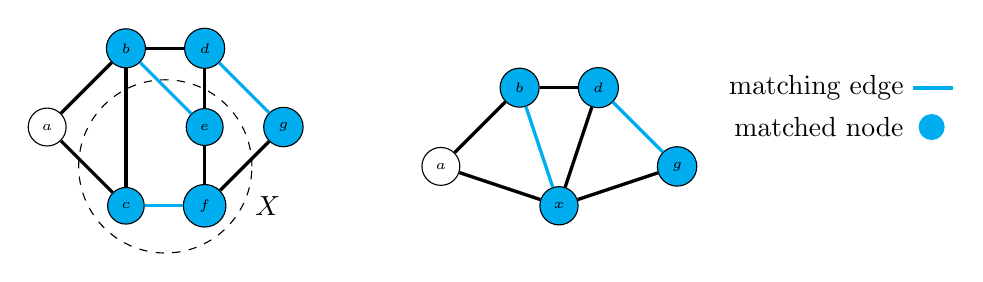
\begin{tikzpicture}
\node[draw, circle] (a) at (0, 0) {\tiny $a$};
\node[draw, circle, fill=cyan] (b) at (1, 1) {\tiny $b$};
\node[draw, circle, fill=cyan] (c) at (1, -1) {\tiny $c$};
\node[draw, circle, fill=cyan] (d) at (2, 1) {\tiny $d$};
\node[draw, circle, fill=cyan] (e) at (2, 0) {\tiny $e$};
\node[draw, circle, fill=cyan] (f) at (2, -1) {\tiny $f$};
\node[draw, circle, fill=cyan] (g) at (3, 0) {\tiny $g$};

\draw[very thick] (a) -- (b);
\draw[very thick] (a) -- (c);
\draw[very thick] (b) -- (c);
\draw[very thick, cyan] (b) -- (e);
\draw[very thick] (b) -- (d);
\draw[very thick, cyan] (c) -- (f);
\draw[very thick] (e) -- (f);
\draw[very thick] (e) -- (d);
\draw[very thick] (f) -- (g);
\draw[very thick, cyan] (d) -- (g);

\draw[dashed] (1.5, -0.5) circle (1.1);
\node at (2.8, -1) {$X$};

\def\x{5}
\def\y{-0.5}

\node[draw, circle] (a) at (\x + 0, \y + 0) {\tiny $a$};
\node[draw, circle, fill=cyan] (b) at (\x + 1, \y + 1) {\tiny $b$};
\node[draw, circle, fill=cyan] (d) at (\x + 2, \y + 1) {\tiny $d$};
\node[draw, circle, fill=cyan] (g) at (\x + 3, \y + 0) {\tiny $g$};
\node[draw, circle, fill=cyan] (x) at (\x + 1.5, \y + -0.5) {\tiny $x$};

\draw[very thick] (a) -- (b);
\draw[very thick] (a) -- (x);
\draw[very thick, cyan] (b) -- (x);
\draw[very thick] (b) -- (d);
\draw[very thick] (x) -- (d);
\draw[very thick] (x) -- (g);
\draw[very thick, cyan] (d) -- (g);

\def\x{11}
\def\y{1}
\draw (\x + 0, \y + -0.5) edge[color = cyan, line width=1.5pt] (\x + 0.5, \y + -0.5) node[text=black, anchor = east] {matching edge};
\node[anchor = east] (z) at (\x + 0, \y + -1) {matched node}; 
\node[circle, fill = cyan, right=0.06cm of z] {};


\end{tikzpicture}
\end{center}

\begin{theorem}
Let $C$ be an alternating odd cycle in $G$ reachable via an alternating path
from some unmatched node. The graph $G$ contains an augmenting path if and only if the graph $G \slash C$ also contains one.
\end{theorem}

\begin{proof}
Let $c$ be the node corresponding to $C$ in $G \slash C$.  \\

First note that if there exists an augmenting path in $G \slash C$ that does not
include node $c$, that path is also an augmenting path in $G$. Therefore we will
focus on the case where the augmenting path in $G \slash C$ includes node $c$.
We will consider 
two cases. \\

\emph{Case 1:} The node $x_1$ from $C$ is unmatched in $G$. Recall that $x_1$ by definition
the only node from the cycle that is not matched to any other node in the cycle. \\

In this case, node $c$ is unmatched in $G \slash C$. This is because $x_1$ is unmatched
and all other nodes in $C$ are already matched to a node within $C$. Hence there cannot be
matching edges exiting node $c$ after the contraction. 
As $c$ is unmatched, any augmenting path in $G \slash C$ that includes node $c$, must 
end on it (an unmatched node can only be an endpoint of an augmenting path). When we unfold
the cycle, this augmenting path will be an alternating path in $G$ from an unmatched node in $G$ to
some node in the cycle $C$. If that node is $x_1$, since $x_1$ is unmatched, that path is
augmenting in $G$. If it is any other node we can extend it by following the cycle
(starting with a matched edge) until we reach $x_1$. In any case we get an augmenting
path in $G$. The following figure illustrates this.

\vspace{0.5cm}

\begin{center}
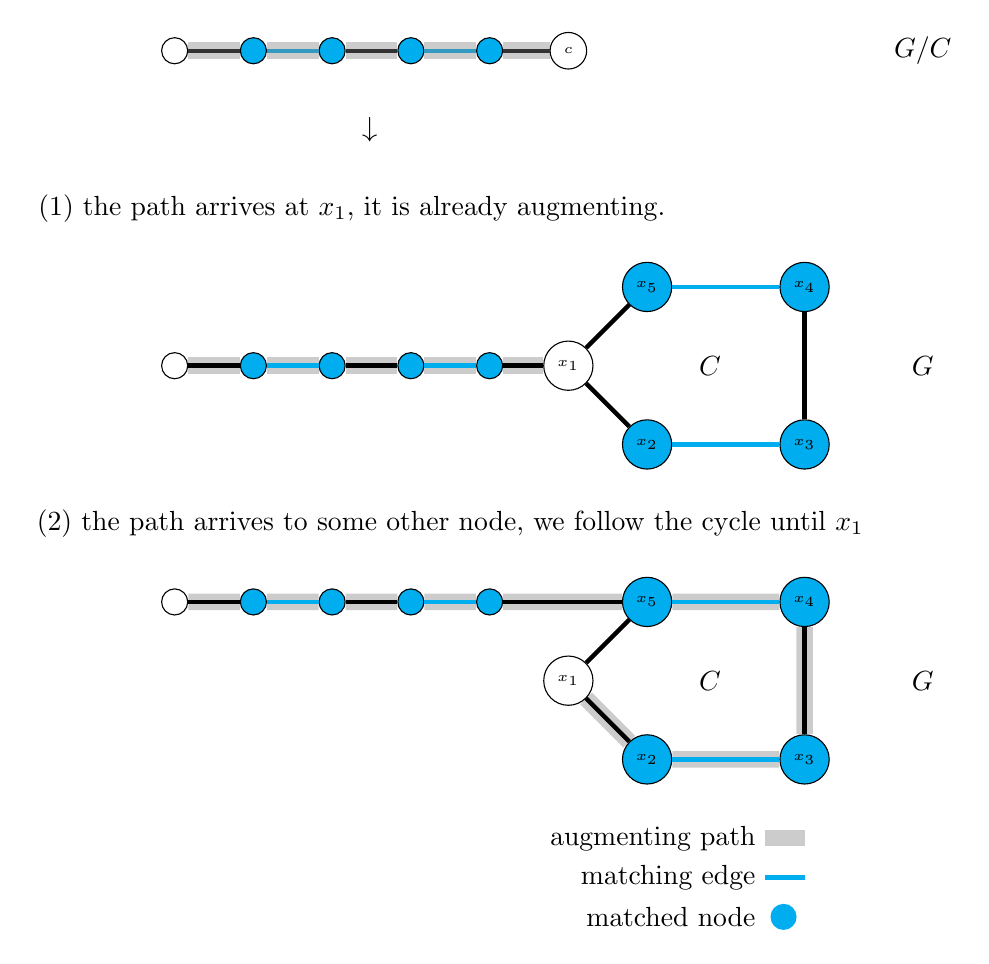
\begin{tikzpicture}
\def\x{-5}

\node[draw, circle] (a) at (\x+0, 0) {};
\node[draw, circle, fill=cyan] (b) at (\x+1, 0) {};
\node[draw, circle, fill=cyan] (c) at (\x+2, 0) {};
\node[draw, circle, fill=cyan] (d) at (\x+3, 0) {};
\node[draw, circle, fill=cyan] (e) at (\x+4, 0) {};
\node[draw, circle] (f) at (\x+5, 0) {\tiny $c$};

\draw[ultra thick] (a) -- (b);
\draw[ultra thick, cyan] (b) -- (c);
\draw[ultra thick] (c) -- (d);
\draw[ultra thick, cyan] (d) -- (e);
\draw[ultra thick] (e) -- (f);

\node[rotate=90] at (\x+2.5, -1) {$\leftarrow$};
\draw[gray, opacity = 0.4, line width=6pt] (a) -- (b) -- (c) -- (d) -- (e) -- (f);

\node at (\x+9.5, 0) {$G \slash C$};
\def\y{-2}

\node at (\x+6.8, -2 + \y) {$C$};
\node at (\x+6.8, -6 + \y) {$C$};
\node at (\x+9.5, -2 + \y) {$G$};
\node at (\x+9.5, -6 + \y) {$G$};

\node[draw, circle] (a) at (\x+0, -2 + \y) {};
\node[draw, circle, fill=cyan] (b) at (\x+1, -2 + \y) {};
\node[draw, circle, fill=cyan] (c) at (\x+2, -2 + \y) {};
\node[draw, circle, fill=cyan] (d) at (\x+3, -2 + \y) {};
\node[draw, circle, fill=cyan] (e) at (\x+4, -2 + \y) {};

\node[draw, circle] (f) at (\x+5, -2 + \y) {\tiny $x_1$};
\node[draw, circle, fill=cyan] (g) at (\x+6, -1 + \y) {\tiny $x_5$};
\node[draw, circle, fill=cyan] (h) at (\x+8, -1 + \y) {\tiny $x_4$};
\node[draw, circle, fill=cyan] (i) at (\x+8, -3 + \y) {\tiny $x_3$};
\node[draw, circle, fill=cyan] (j) at (\x+6, -3 + \y) {\tiny $x_2$};

\draw[gray, opacity = 0.4, line width=6pt] (a) -- (b) -- (c) -- (d) -- (e) -- (f);

\draw[ultra thick] (a) -- (b);
\draw[ultra thick, cyan] (b) -- (c);
\draw[ultra thick] (c) -- (d);
\draw[ultra thick, cyan] (d) -- (e);
\draw[ultra thick] (e) -- (f);

\draw[ultra thick] (f) -- (g);
\draw[ultra thick, cyan] (g) -- (h);
\draw[ultra thick] (h) -- (i);
\draw[ultra thick, cyan] (i) -- (j);
\draw[ultra thick] (j) -- (f);

%\node at (2.5, -3.5) {or};

\node at (-2.75,+\y) {(1) the path arrives at $x_1$, it is already augmenting.};

\def\y{-6}

\node[draw, circle] (a) at (\x + 0, -1 + \y) {};
\node[draw, circle, fill=cyan] (b) at (\x +1, -1 + \y) {};
\node[draw, circle, fill=cyan] (c) at (\x+2, -1 + \y) {};
\node[draw, circle, fill=cyan] (d) at (\x+3, -1 + \y) {};
\node[draw, circle, fill=cyan] (e) at (\x+4, -1 + \y) {};

\node[draw, circle] (f) at (\x+5, -2 + \y) {\tiny $x_1$};
\node[draw, circle, fill=cyan] (g) at (\x+6, -1 + \y) {\tiny $x_5$};
\node[draw, circle, fill=cyan] (h) at (\x+8, -1 + \y) {\tiny $x_4$};
\node[draw, circle, fill=cyan] (i) at (\x+8, -3 + \y) {\tiny $x_3$};
\node[draw, circle, fill=cyan] (j) at (\x+6, -3 + \y) {\tiny $x_2$};

\draw[gray, opacity = 0.4, line width=6pt] (a) -- (b) -- (c) -- (d) -- (e) -- (g) -- (h) -- (i) -- (j) -- (f);

\draw[ultra thick] (a) -- (b);
\draw[ultra thick, cyan] (b) -- (c);
\draw[ultra thick] (c) -- (d);
\draw[ultra thick, cyan] (d) -- (e);
\draw[ultra thick] (e) -- (g);

\draw[ultra thick] (f) -- (g);
\draw[ultra thick, cyan] (g) -- (h);
\draw[ultra thick] (h) -- (i);
\draw[ultra thick, cyan] (i) -- (j);
\draw[ultra thick] (j) -- (f);

\node at (-1.5, 0 + \y) {(2) the path arrives to some other node, we follow the cycle until $x_1$};

\draw (\x +7.5, -4 + \y) edge[color = gray, opacity = 0.4, line width=6pt] (\x+8, -4 + \y) node[text=black, anchor = east] {augmenting path};
\draw (\x+7.5, -4.5 + \y) edge[color = cyan, line width=1.5pt] (\x+8, -4.5 + \y) node[text=black, anchor = east] {matching edge};
\node[anchor = east] (z) at (\x+7.5, -5 + \y) {matched node}; 
\node[circle, fill = cyan, right=0.06cm of z] {};
\end{tikzpicture}
\end{center}

\emph{Case 2:} The node $x_1$ from $C$ is matched in $G$. By hypothesis the cycle
$C$ is reachable via an alternating path from some unmatched node, say $x$. Therefore, since
the path is an alternating path from $x$ to $x_1$, if we reverse its edges we still get a valid matching
of the same size, except that now $x_1$ is unmatched. Then we can apply the previous case
to this new matching and cycle $C$ because $x_1$ has become
unmatched. \\

This is actually enough to compute a matching of larger size. However the astute reader
might notice that in this case we did not really get an augmenting path relative
to the original matching (because we reversed the edge on the path from $x$ to $x_1$).
However it is not hard to see that by reversing those edges back after finding an augmenting path
in $G \slash C$ we can actually continue to extend that path by following the cycle as 
before but then, instead of stopping at $x_1$ (which is not unmatched anymore)
we continue following the path from $x_1$ to $x$ and obtain a path relative to the
original matching. This will be illustrated in the next example.

\end{proof}

This theorem gives us an algorithm to compute augmenting paths. We start on $G$ and 
compute an alternating odd cycle in $G$. This can be achieved using a \textsf{BFS}
from the set of unmatched nodes and finding an edge $e = (u, v)$ between two nodes at the same level.
Tracing back the parents of $u$ and $v$ will lead to one of two situations: either $u$ and $v$ are 
two distinct sources, in which case we have found an augmenting path; or at some point we reach a common
ancestor. This ancestor together with the paths linking it to $u$ and $v$ forms an alternating odd cycle.
Since the graph becomes smaller at each contraction, this process must stop at some point.

We will illustrate the execution of the algorithm on the following graph.

\begin{center}
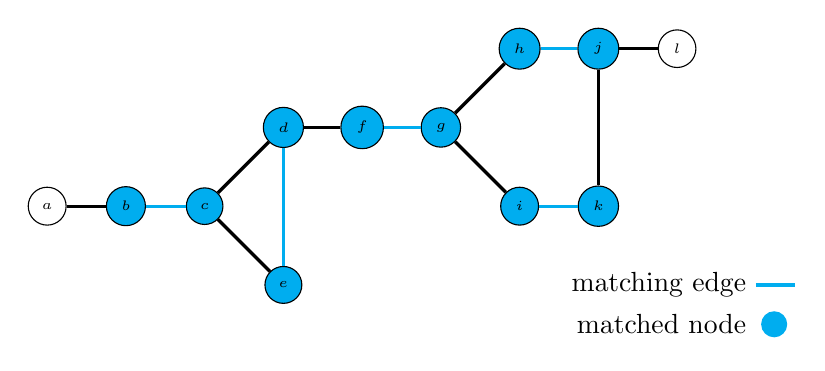
\begin{tikzpicture}
\def\x{0}
\def\y{0}

\node[draw, circle] (a) at (\x + 0, \y + 0) {\tiny $a$};
\node[draw, circle, fill=cyan] (b) at (\x + 1, \y + 0) {\tiny $b$};
\node[draw, circle, fill=cyan] (c) at (\x + 2, \y + 0) {\tiny $c$};
\node[draw, circle, fill=cyan] (d) at (\x + 3, \y + 1) {\tiny $d$};
\node[draw, circle, fill=cyan] (e) at (\x + 3, \y + -1){\tiny $e$};
\node[draw, circle, fill=cyan] (f) at (\x + 4, \y + 1) {\tiny $f$};
\node[draw, circle, fill=cyan] (g) at (\x + 5, \y + 1) {\tiny $g$};
\node[draw, circle, fill=cyan] (h) at (\x + 6, \y + 2) {\tiny $h$};
\node[draw, circle, fill=cyan] (i) at (\x + 6, \y + 0) {\tiny $i$};
\node[draw, circle, fill=cyan] (j) at (\x + 7, \y + 2) {\tiny $j$};
\node[draw, circle, fill=cyan] (k) at (\x + 7, \y + 0) {\tiny $k$};
\node[draw, circle] (l) at (\x + 8, \y + 2) {\tiny $l$};

\draw[very thick] (a) -- (b);
\draw[very thick, cyan] (b) -- (c);
\draw[very thick] (c) -- (d);
\draw[very thick] (c) -- (e);
\draw[very thick, cyan] (e) -- (d);
\draw[very thick] (d) -- (f);
\draw[very thick, cyan] (f) -- (g);
\draw[very thick] (g) -- (h);
\draw[very thick] (g) -- (i);
\draw[very thick, cyan] (h) -- (j);
\draw[very thick, cyan] (i) -- (k);
\draw[very thick] (k) -- (j);
\draw[very thick] (j) -- (l);

\def\x{9}
\def\y{-0.5}
\draw (\x + 0, \y + -0.5) edge[color = cyan, line width=1.5pt] (\x + 0.5, \y + -0.5) node[text=black, anchor = east] {matching edge};
\node[anchor = east] (z) at (\x + 0, \y + -1) {matched node}; 
\node[circle, fill = cyan, right=0.06cm of z] {};


\end{tikzpicture}
\end{center} 

Perform a \textsf{BFS} from the set of unmatched nodes $a$ and $l$ and look
for an edge between two nodes in the same level. In this case we find edge $(d, e)$
(it does not need to be a matching edge). Such an edge yields either an alternating
odd cycle or an augmenting path depending on whether they trace back to a common
ancestor or two distinct sources from the \textsf{BFS}.
This can be computed by going up the tree following the parents of
$d$ and $e$. We either reach a common ancestor or two sources. In this case we the common
ancestor $c$ and get the cycle $C = \{ c, d, e \}$. 


\begin{center}
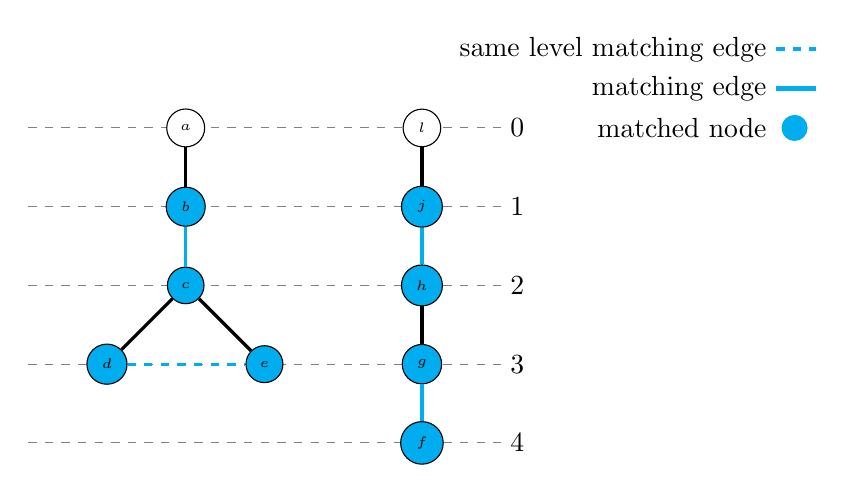
\begin{tikzpicture}

\def\x{0}
\def\y{-2}

\draw[dashed, gray] (\x + -2, \y+ 0) -- (\x + 4, \y + 0) node[black, anchor = west] {$0$};
\draw[dashed, gray] (\x + -2, \y+ -1) -- (\x + 4, \y + -1) node[black, anchor = west] {$1$};
\draw[dashed, gray] (\x + -2, \y+ -2) -- (\x + 4, \y + -2) node[black, anchor = west] {$2$};
\draw[dashed, gray] (\x + -2, \y+ -3) -- (\x + 4, \y + -3) node[black, anchor = west] {$3$};
\draw[dashed, gray] (\x + -2, \y+ -4) -- (\x + 4, \y + -4) node[black, anchor = west] {$4$};


\node[draw, circle, fill=white] (a) at (\x + 0, \y + 0) {\tiny $a$};
\node[draw, circle, fill=cyan] (b) at (\x + 0, \y + -1) {\tiny $b$};
\node[draw, circle, fill=cyan] (c) at (\x + 0, \y + -2) {\tiny $c$};
\node[draw, circle, fill=cyan] (d) at (\x + -1, \y + -3) {\tiny $d$};
\node[draw, circle, fill=cyan] (e) at (\x + 1, \y + -3) {\tiny $e$};

\draw[very thick] (a) -- (b);
\draw[very thick, cyan] (b) -- (c);
\draw[very thick] (c) -- (d);
\draw[very thick] (c) -- (e);
\draw[very thick, dashed, cyan] (d) -- (e);

\node[draw, circle, fill=white] (l) at (\x + 3, \y + 0) {\tiny $l$};
\node[draw, circle, fill=cyan] (j) at (\x + 3, \y + -1) {\tiny $j$};
\node[draw, circle, fill=cyan] (h) at (\x + 3, \y + -2) {\tiny $h$};
\node[draw, circle, fill=cyan] (g) at (\x + 3, \y + -3) {\tiny $g$};
\node[draw, circle, fill=cyan] (f) at (\x + 3, \y + -4) {\tiny $f$};

\draw[very thick] (l) -- (j);
\draw[very thick, cyan] (j) -- (h);
\draw[very thick] (h) -- (g);
\draw[very thick, cyan] (g) -- (f);

\def\x{7.5}
\def\y{-1}
\draw (\x + 0, \y) edge[dashed, color = cyan, line width=1.5pt] (\x + 0.5, \y) node[text=black, anchor = east] {same level matching edge};
\draw (\x + 0, \y + -0.5) edge[color = cyan, line width=1.5pt] (\x + 0.5, \y + -0.5) node[text=black, anchor = east] {matching edge};
\node[anchor = east] (z) at (\x + 0, \y + -1) {matched node}; 
\node[circle, fill = cyan, right=0.06cm of z] {};


%\node[text width=3cm] at (0.5 + \x, -3.65 + \y) {\tiny edge between nodes \\ in the same level};

\end{tikzpicture}
\end{center}

Since node $c$ is matched, we reverse the matching on the
path from $a$ to $c$. Then we know that the result graph has
an augmenting path if and only if $G \slash C$ has an augmenting path.

\begin{center}
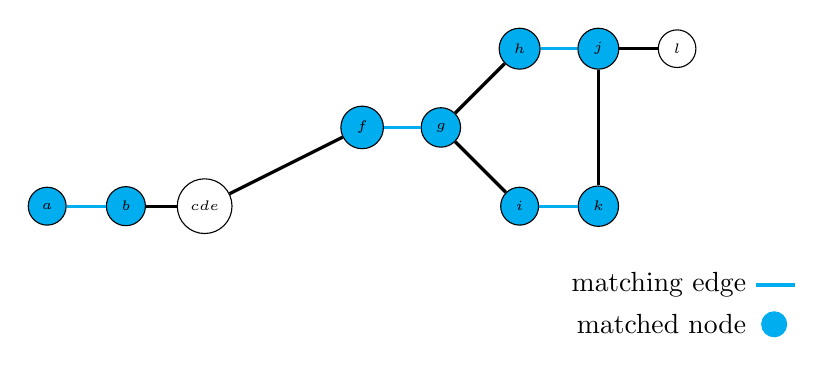
\begin{tikzpicture}
\def\x{0}
\def\y{0}

\node[draw, circle, fill=cyan] (a) at (\x + 0, \y + 0) {\tiny $a$};
\node[draw, circle, fill=cyan] (b) at (\x + 1, \y + 0) {\tiny $b$};
\node[draw, circle] (cde) at (\x + 2, \y + 0) {\tiny $cde$};
\node[draw, circle, fill=cyan] (f) at (\x + 4, \y + 1) {\tiny $f$};
\node[draw, circle, fill=cyan] (g) at (\x + 5, \y + 1) {\tiny $g$};
\node[draw, circle, fill=cyan] (h) at (\x + 6, \y + 2) {\tiny $h$};
\node[draw, circle, fill=cyan] (i) at (\x + 6, \y + 0) {\tiny $i$};
\node[draw, circle, fill=cyan] (j) at (\x + 7, \y + 2) {\tiny $j$};
\node[draw, circle, fill=cyan] (k) at (\x + 7, \y + 0) {\tiny $k$};
\node[draw, circle] (l) at (\x + 8, \y + 2) {\tiny $l$};

\draw[very thick, cyan] (a) -- (b);
\draw[very thick] (b) -- (cde);
\draw[very thick] (cde) -- (f);
\draw[very thick, cyan] (f) -- (g);
\draw[very thick] (g) -- (h);
\draw[very thick] (g) -- (i);
\draw[very thick, cyan] (h) -- (j);
\draw[very thick, cyan] (i) -- (k);
\draw[very thick] (k) -- (j);
\draw[very thick] (j) -- (l);

\def\x{9}
\def\y{-0.5}
\draw (\x + 0, \y + -0.5) edge[color = cyan, line width=1.5pt] (\x + 0.5, \y + -0.5) node[text=black, anchor = east] {matching edge};
\node[anchor = east] (z) at (\x + 0, \y + -1) {matched node}; 
\node[circle, fill = cyan, right=0.06cm of z] {};


\end{tikzpicture}
\end{center}

We perform a new \textsf{BFS} on $G \slash C$ from the unmatched nodes $cde$ and $l$. Here we find
edge $(g, h)$ between two nodes of the same level. By tracing back the parents we
reach nodes $cde$ and $l$. This means that we have found and augmenting path
$(cde, f, g, h, j, l)$ on $G \slash C$.

\begin{center}
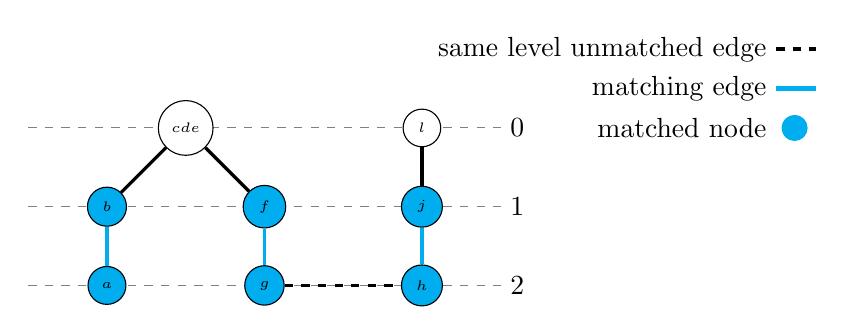
\begin{tikzpicture}

\def\x{0}
\def\y{-2}

\draw[dashed, gray] (\x + -2, \y+ 0) -- (\x + 4, \y + 0) node[black, anchor = west] {$0$};
\draw[dashed, gray] (\x + -2, \y+ -1) -- (\x + 4, \y + -1) node[black, anchor = west] {$1$};
\draw[dashed, gray] (\x + -2, \y+ -2) -- (\x + 4, \y + -2) node[black, anchor = west] {$2$};


\node[draw, circle, fill=white] (cde) at (\x + 0, \y + 0) {\tiny $cde$};
\node[draw, circle, fill=cyan] (b) at (\x + -1, \y + -1) {\tiny $b$};
\node[draw, circle, fill=cyan] (f) at (\x + 1, \y + -1) {\tiny $f$};
\node[draw, circle, fill=cyan] (a) at (\x + -1, \y + -2) {\tiny $a$};
\node[draw, circle, fill=cyan] (g) at (\x + 1, \y + -2) {\tiny $g$};

\draw[very thick] (cde) -- (b);
\draw[very thick] (cde) -- (f);
\draw[very thick, cyan] (b) -- (a);
\draw[very thick, cyan] (f) -- (g);

\node[draw, circle, fill=white] (l) at (\x + 3, \y + 0) {\tiny $l$};
\node[draw, circle, fill=cyan] (j) at (\x + 3, \y + -1) {\tiny $j$};
\node[draw, circle, fill=cyan] (h) at (\x + 3, \y + -2) {\tiny $h$};

\draw[very thick] (l) -- (j);
\draw[very thick, cyan] (j) -- (h);

\draw[very thick, dashed] (g) -- (h);
%\node[text width=3cm] at (0.5 + \x, -3.65 + \y) {\tiny edge between nodes \\ in the same level};

\def\x{7.5}
\def\y{-1}
\draw (\x + 0, \y) edge[dashed, line width=1.5pt] (\x + 0.5, \y) node[text=black, anchor = east] {same level unmatched edge};
\draw (\x + 0, \y + -0.5) edge[color = cyan, line width=1.5pt] (\x + 0.5, \y + -0.5) node[text=black, anchor = east] {matching edge};
\node[anchor = east] (z) at (\x + 0, \y + -1) {matched node}; 
\node[circle, fill = cyan, right=0.06cm of z] {};



\end{tikzpicture}
\end{center}

Unfolding the path we get a path from $d$ to $l$ on $G$ as shown in the figure.
Then we follow the cycle starting with a matching edge until we reach $c$, the
unmatched node of the cycle. This yields an augmenting path in $G$.

\begin{center}
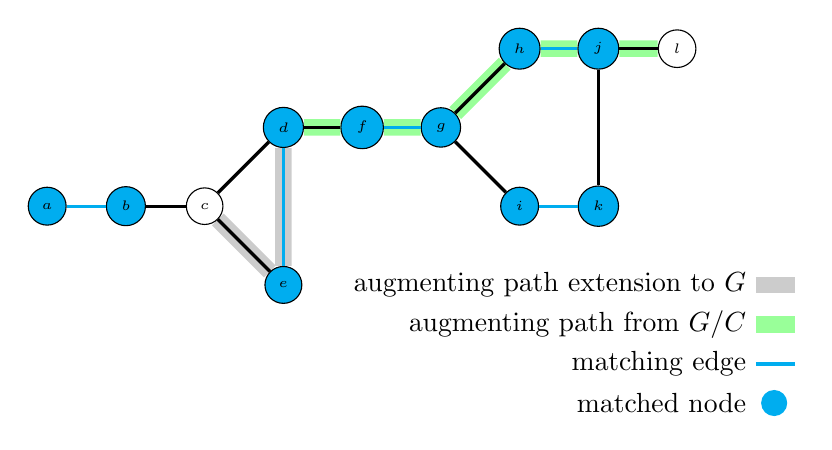
\begin{tikzpicture}
\def\x{0}
\def\y{0}

\node[draw, circle, fill=cyan] (a) at (\x + 0, \y + 0) {\tiny $a$};
\node[draw, circle, fill=cyan] (b) at (\x + 1, \y + 0) {\tiny $b$};
\node[draw, circle] (c) at (\x + 2, \y + 0) {\tiny $c$};
\node[draw, circle, fill=cyan] (d) at (\x + 3, \y + 1) {\tiny $d$};
\node[draw, circle, fill=cyan] (e) at (\x + 3, \y + -1){\tiny $e$};
\node[draw, circle, fill=cyan] (f) at (\x + 4, \y + 1) {\tiny $f$};
\node[draw, circle, fill=cyan] (g) at (\x + 5, \y + 1) {\tiny $g$};
\node[draw, circle, fill=cyan] (h) at (\x + 6, \y + 2) {\tiny $h$};
\node[draw, circle, fill=cyan] (i) at (\x + 6, \y + 0) {\tiny $i$};
\node[draw, circle, fill=cyan] (j) at (\x + 7, \y + 2) {\tiny $j$};
\node[draw, circle, fill=cyan] (k) at (\x + 7, \y + 0) {\tiny $k$};
\node[draw, circle] (l) at (\x + 8, \y + 2) {\tiny $l$};

\draw[green, opacity = 0.4, line width=6pt] (d) -- (f) -- (g) --  (h) -- (j) -- (l);
\draw[gray, opacity = 0.4, line width=6pt] (d) -- (e) -- (c);
%\draw[orange, opacity = 0.4, line width=6pt] (c) -- (b) -- (a);

\draw[very thick, cyan] (a) -- (b);
\draw[very thick] (b) -- (c);
\draw[very thick] (c) -- (d);
\draw[very thick] (c) -- (e);
\draw[very thick, cyan] (e) -- (d);
\draw[very thick] (d) -- (f);
\draw[very thick, cyan] (f) -- (g);
\draw[very thick] (g) -- (h);
\draw[very thick] (g) -- (i);
\draw[very thick, cyan] (h) -- (j);
\draw[very thick, cyan] (i) -- (k);
\draw[very thick] (k) -- (j);
\draw[very thick] (j) -- (l);

\def\x{9}
\def\y{-1.5}
\draw (\x + 0, \y + -0.5) edge[color = cyan, line width=1.5pt] (\x + 0.5, \y + -0.5) node[text=black, anchor = east] {matching edge};
\node[anchor = east] (z) at (\x + 0, \y + -1) {matched node}; 
\node[circle, fill = cyan, right=0.06cm of z] {};
\draw (\x + 0, \y + 0) edge[color = green, opacity = 0.4, line width=6pt] (\x + 0.5, \y + 0) node[text=black, anchor = east] {augmenting path from $G \slash C$};
\draw (\x + 0, \y + 0.5) edge[color = gray, opacity = 0.4, line width=6pt] (\x + 0.5, \y + 0.5) node[text=black, anchor = east] {augmenting path extension to $G$};


\end{tikzpicture}
\end{center} 

As we observed at the end of the previous proof, this path is not an
augmenting path for the initial matching. It is an augmenting path
for the matching where $b$ is matched to $a$ instead of $c$. But if we
want we can actually recover an augmenting path relative to the original
matching by reversing again the edges on the path $(a, b, c)$ and extending
the previous path until $a$ as shown next.

\begin{center}
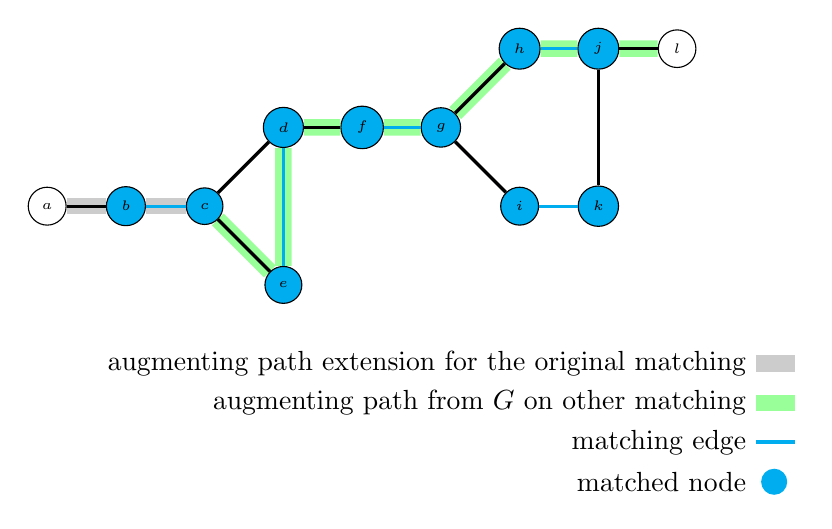
\begin{tikzpicture}
\def\x{0}
\def\y{0}

\node[draw, circle] (a) at (\x + 0, \y + 0) {\tiny $a$};
\node[draw, circle, fill=cyan] (b) at (\x + 1, \y + 0) {\tiny $b$};
\node[draw, circle, fill=cyan] (c) at (\x + 2, \y + 0) {\tiny $c$};
\node[draw, circle, fill=cyan] (d) at (\x + 3, \y + 1) {\tiny $d$};
\node[draw, circle, fill=cyan] (e) at (\x + 3, \y + -1){\tiny $e$};
\node[draw, circle, fill=cyan] (f) at (\x + 4, \y + 1) {\tiny $f$};
\node[draw, circle, fill=cyan] (g) at (\x + 5, \y + 1) {\tiny $g$};
\node[draw, circle, fill=cyan] (h) at (\x + 6, \y + 2) {\tiny $h$};
\node[draw, circle, fill=cyan] (i) at (\x + 6, \y + 0) {\tiny $i$};
\node[draw, circle, fill=cyan] (j) at (\x + 7, \y + 2) {\tiny $j$};
\node[draw, circle, fill=cyan] (k) at (\x + 7, \y + 0) {\tiny $k$};
\node[draw, circle] (l) at (\x + 8, \y + 2) {\tiny $l$};

\draw[green, opacity = 0.4, line width=6pt] (d) -- (f) -- (g) --  (h) -- (j) -- (l);
\draw[green, opacity = 0.4, line width=6pt] (d) -- (e) -- (c);
\draw[gray, opacity = 0.4, line width=6pt] (c) -- (b) -- (a);

\draw[very thick] (a) -- (b);
\draw[very thick, cyan] (b) -- (c);
\draw[very thick] (c) -- (d);
\draw[very thick] (c) -- (e);
\draw[very thick, cyan] (e) -- (d);
\draw[very thick] (d) -- (f);
\draw[very thick, cyan] (f) -- (g);
\draw[very thick] (g) -- (h);
\draw[very thick] (g) -- (i);
\draw[very thick, cyan] (h) -- (j);
\draw[very thick, cyan] (i) -- (k);
\draw[very thick] (k) -- (j);
\draw[very thick] (j) -- (l);

\def\x{9}
\def\y{-2.5}
\draw (\x + 0, \y + -0.5) edge[color = cyan, line width=1.5pt] (\x + 0.5, \y + -0.5) node[text=black, anchor = east] {matching edge};
\node[anchor = east] (z) at (\x + 0, \y + -1) {matched node}; 
\node[circle, fill = cyan, right=0.06cm of z] {};
\draw (\x + 0, \y + 0) edge[color = green, opacity = 0.4, line width=6pt] (\x + 0.5, \y + 0) node[text=black, anchor = east] {augmenting path from $G$ on other matching};
\draw (\x + 0, \y + 0.5) edge[color = gray, opacity = 0.4, line width=6pt] (\x + 0.5, \y + 0.5) node[text=black, anchor = east] {augmenting path extension for the original matching};


\end{tikzpicture}
\end{center} 

I will describe and implementation of the algorithm when I find the time. For now it is a good exercise for you
to try to implement it yourself. Note that there can we several contractions during the execution. I will also
try to add examples where this happens to make it more clear what happens in this case. Contractions are not always
easy to implement because unfolding might be tricky.

% 
% \begin{center}
% \begin{tikzpicture}
% \node[draw, circle] (a) at (0, 0) {\tiny $x_1$};
% \node[draw, circle] (b) at (1, -1) {\tiny $x_2$};
% \node[draw, circle] (c) at (3, -1) {\tiny $x_3$};
% \node[draw, circle] (d) at (3, 1) {\tiny $x_4$};
% \node[draw, circle] (e) at (1, 1) {\tiny $x_5$};
% \draw[very thick] (a) -- (b);
% \draw[very thick, cyan] (b) -- (c);
% \draw[very thick] (c) -- (d);
% \draw[very thick, cyan] (d) -- (e);
% \draw[very thick] (e) -- (a);
% 
% \draw[very thick] (a) -- (-0.5, -0.5);
% \draw[very thick] (a) -- (-0.5, 0.5);
% 
% \draw[very thick] (e) -- (1 -0.5, 1+0.5);
% \draw[very thick] (e) -- (1 +0.5, 1+0.5);
% 
% \draw[very thick] (d) -- (3, 1+0.7);
% \draw[very thick] (d) -- (3+0.7, 1);
% 
% \draw[very thick] (c) -- (3, -1-0.7);
% \draw[very thick] (c) -- (3+0.7, -1);
% 
% \draw[very thick] (b) -- (1 -0.5, -1-0.5);
% \draw[very thick] (b) -- (1 +0.5, -1-0.5);
% \end{tikzpicture}
% \end{center}
% 
% 
% 
% 
% First observe that 
% $c$ is unmatched in $G \slash C$. This is because $v_1$ is unmatched and all
% of the others are matched already to some node of the cycle. Therefore there cannot
% be matching edge from a node in $C$ to a node outside $C$.
% Now, if $G \slash C$ has an augmentin path that does not include node
% $c$, then that will also be an augmenting path in $G$. All that remains
% to show is that from an augmenting path in $G \slash C$ that includes node
% $c$ we can build an augmenting path in $G$.
% 
% Let $p$ be any augmenting path in $G \slash C$ that includes node $c$. By
% what we observe before, $c$ is unmatched in $G \slash C$. Therefore $c$ must
% be an endpoint of $p$ (only the endpoints in an agumenting path are
% unmatched). When we unfold the cycle and get back to $G$, the path $p$
% will be an alternating path from an unmatched node and ending in some
% node of the cycle $C$ via an unmatched edge. Then we can just expand the
% path by following the cycle (starting with a matching edge) 
% until we reach $v_1$. Since $v_1$ is unmatched
% and the path starts at an unmatched node, the path must be augmenting.
% 
% 
% \begin{center}
% \begin{figure}
% \begin{tikzpicture}
% \node[draw, circle] (a) at (0, 0) {};
% \node[draw, circle, fill=cyan] (b) at (1, 0) {};
% \node[draw, circle, fill=cyan] (c) at (2, 0) {};
% \node[draw, circle, fill=cyan] (d) at (3, 0) {};
% \node[draw, circle, fill=cyan] (e) at (4, 0) {};
% \node[draw, circle] (f) at (5, 0) {\tiny $c$};
% 
% \draw[ultra thick] (a) -- (b);
% \draw[ultra thick, cyan] (b) -- (c);
% \draw[ultra thick] (c) -- (d);
% \draw[ultra thick, cyan] (d) -- (e);
% \draw[ultra thick] (e) -- (f);
% 
% \node[rotate=90] at (2.5, -1) {$\leftarrow$};
% \draw[gray, opacity = 0.4, line width=6pt] (a) -- (b) -- (c) -- (d) -- (e) -- (f);
% 
% \node at (9.5, 0) {$G \slash C$};
% \def\y{-1}
% 
% \node at (6.8, -2 + \y) {$C$};
% \node at (6.8, -5 + \y) {$C$};
% \node at (9.5, -3.5 + \y) {$G$};
% 
% 
% \node[draw, circle] (a) at (0, -2 + \y) {};
% \node[draw, circle, fill=cyan] (b) at (1, -2 + \y) {};
% \node[draw, circle, fill=cyan] (c) at (2, -2 + \y) {};
% \node[draw, circle, fill=cyan] (d) at (3, -2 + \y) {};
% \node[draw, circle, fill=cyan] (e) at (4, -2 + \y) {};
% 
% \node[draw, circle] (f) at (5, -2 + \y) {\tiny $v_1$};
% \node[draw, circle, fill=cyan] (g) at (6, -1 + \y) {\tiny $v_5$};
% \node[draw, circle, fill=cyan] (h) at (8, -1 + \y) {\tiny $v_4$};
% \node[draw, circle, fill=cyan] (i) at (8, -3 + \y) {\tiny $v_3$};
% \node[draw, circle, fill=cyan] (j) at (6, -3 + \y) {\tiny $v_2$};
% 
% \draw[gray, opacity = 0.4, line width=6pt] (a) -- (b) -- (c) -- (d) -- (e) -- (f);
% 
% \draw[ultra thick] (a) -- (b);
% \draw[ultra thick, cyan] (b) -- (c);
% \draw[ultra thick] (c) -- (d);
% \draw[ultra thick, cyan] (d) -- (e);
% \draw[ultra thick] (e) -- (f);
% 
% \draw[ultra thick] (f) -- (g);
% \draw[ultra thick, cyan] (g) -- (h);
% \draw[ultra thick] (h) -- (i);
% \draw[ultra thick, cyan] (i) -- (j);
% \draw[ultra thick] (j) -- (f);
% 
% %\node at (2.5, -3.5) {or};
% 
% \node at (-1.5, -2) {(1)};
% 
% \def\y{-4}
% 
% \node[draw, circle] (a) at (0, -1 + \y) {};
% \node[draw, circle, fill=cyan] (b) at (1, -1 + \y) {};
% \node[draw, circle, fill=cyan] (c) at (2, -1 + \y) {};
% \node[draw, circle, fill=cyan] (d) at (3, -1 + \y) {};
% \node[draw, circle, fill=cyan] (e) at (4, -1 + \y) {};
% 
% \node[draw, circle] (f) at (5, -2 + \y) {\tiny $v_1$};
% \node[draw, circle, fill=cyan] (g) at (6, -1 + \y) {\tiny $v_5$};
% \node[draw, circle, fill=cyan] (h) at (8, -1 + \y) {\tiny $v_4$};
% \node[draw, circle, fill=cyan] (i) at (8, -3 + \y) {\tiny $v_3$};
% \node[draw, circle, fill=cyan] (j) at (6, -3 + \y) {\tiny $v_2$};
% 
% \draw[gray, opacity = 0.4, line width=6pt] (a) -- (b) -- (c) -- (d) -- (e) -- (g) -- (h) -- (i) -- (j) -- (f);
% 
% \draw[ultra thick] (a) -- (b);
% \draw[ultra thick, cyan] (b) -- (c);
% \draw[ultra thick] (c) -- (d);
% \draw[ultra thick, cyan] (d) -- (e);
% \draw[ultra thick] (e) -- (g);
% 
% \draw[ultra thick] (f) -- (g);
% \draw[ultra thick, cyan] (g) -- (h);
% \draw[ultra thick] (h) -- (i);
% \draw[ultra thick, cyan] (i) -- (j);
% \draw[ultra thick] (j) -- (f);
% 
% \node at (-1.5, -1 + \y) {(2)};
% 
% \draw (7.5, -4 + \y) edge[color = gray, opacity = 0.4, line width=6pt] (8, -4 + \y) node[text=black, anchor = east] {augmenting path};
% \draw (7.5, -4.5 + \y) edge[color = cyan, line width=1.5pt] (8, -4.5 + \y) node[text=black, anchor = east] {matching edge};
% \node[anchor = east] (z) at (7.5, -5 + \y) {matched node}; 
% \node[circle, fill = cyan, right=0.06cm of z] {};
% \end{tikzpicture}
% \caption{Building an augmenting path in $G$ from an augmenting path in $G \slash C$. On top we see
% a case where the path in $G \slash C$ ends in $v_1$. In this case the path is already augmenting
% in $G$. On the other case we still need to complete it. For this we follow the cycle in the
% direction of the first matched edge until we reach $v_1$.}
% \end{figure}
% \end{center}
% 
% \end{proof}
% 
% 
% 
% \newpage
% 
% 
% 
% 
% 
% 
% 
% 
% 
% 
% 
% 
% 
% 
% 
% 
% 
% \textbf{TODO: add example}
% 
% \begin{center}
% \begin{tikzpicture}
% \node[draw, circle] (a) at (0, 0) {\tiny $v_1$};
% \node[draw, circle] (b) at (1, -1) {\tiny $v_2$};
% \node[draw, circle] (c) at (3, -1) {\tiny $v_3$};
% \node[draw, circle] (d) at (3, 1) {\tiny $v_4$};
% \node[draw, circle] (e) at (1, 1) {\tiny $v_5$};
% \draw[very thick] (a) -- (b);
% \draw[very thick] (b) edge node {\footnotesize $||$} (c);
% \match{d}{e}
% \draw[very thick] (c) -- (d);
% \draw[very thick] (e) -- (a);
% \end{tikzpicture}
% \end{center}
% 
% If you extend  changed it to allow to visit each node twice, one coming from a dirt edge and the other from a water edge, then you
% find some paths that contain cycles. \\
% 
% 
% 
% Since each river had length 1, there will be no node that is connected to more than one river. Therefore the rivers from a matching in the graph.
% And the goal is to find a path from two unmatched nodes that alternates between dirt and water. In other words, you need to find an
% \emph{augmenting path}. \\
% 
% \begin{definition}
% A cycle $C = (v_1, v_2, v_3, \ldots, v_k)$ is said to be an \emph{alternating odd cycle} if $k$ is odd,
% $v_1$ is unmatched and its edges alternate between matched and unmatched.
% \end{definition}
% 
% \begin{center}
% \begin{tikzpicture}
% \node[draw, circle] (a) at (0, 0) {\tiny $v_1$};
% \node[draw, circle] (b) at (1, -1) {\tiny $v_2$};
% \node[draw, circle] (c) at (3, -1) {\tiny $v_3$};
% \node[draw, circle] (d) at (3, 1) {\tiny $v_4$};
% \node[draw, circle] (e) at (1, 1) {\tiny $v_5$};
% \draw[very thick] (a) -- (b);
% \draw[very thick, cyan] (b) -- (c);
% \draw[very thick] (c) -- (d);
% \draw[very thick, cyan] (d) -- (e);
% \draw[very thick] (e) -- (a);
% \end{tikzpicture}
% \end{center}
% 
% \begin{lemma}
% Let $C$ be an alternating odd cycle in $G$. The graph $G$ contains an augmenting
% path if and only if the graph $G \slash C$ also contains one.
% \end{lemma}
% 
% \begin{proof}
% Let $c$ be the node corresponding to $C$ in $G \slash C$. First observe that 
% $c$ is unmatched in $G \slash C$. This is because $v_1$ is unmatched and all
% of the others are matched already to some node of the cycle. Therefore there cannot
% be matching edge from a node in $C$ to a node outside $C$.
% 
% \begin{center}
% \begin{tikzpicture}
% \node[draw, circle] (a) at (0, 0) {\tiny $v_1$};
% \node[draw, circle] (b) at (1, -1) {\tiny $v_2$};
% \node[draw, circle] (c) at (3, -1) {\tiny $v_3$};
% \node[draw, circle] (d) at (3, 1) {\tiny $v_4$};
% \node[draw, circle] (e) at (1, 1) {\tiny $v_5$};
% \draw[very thick] (a) -- (b);
% \draw[very thick, cyan] (b) -- (c);
% \draw[very thick] (c) -- (d);
% \draw[very thick, cyan] (d) -- (e);
% \draw[very thick] (e) -- (a);
% 
% \draw[very thick] (a) -- (-0.5, -0.5);
% \draw[very thick] (a) -- (-0.5, 0.5);
% 
% \draw[very thick] (e) -- (1 -0.5, 1+0.5);
% \draw[very thick] (e) -- (1 +0.5, 1+0.5);
% 
% \draw[very thick] (d) -- (3, 1+0.7);
% \draw[very thick] (d) -- (3+0.7, 1);
% 
% \draw[very thick] (c) -- (3, -1-0.7);
% \draw[very thick] (c) -- (3+0.7, -1);
% 
% \draw[very thick] (b) -- (1 -0.5, -1-0.5);
% \draw[very thick] (b) -- (1 +0.5, -1-0.5);
% \end{tikzpicture}
% \end{center}
% \end{proof}
% 
% Now, if $G \slash C$ has an augmentin path that does not include node
% $c$, then that will also be an augmenting path in $G$. All that remains
% to show is that from an augmenting path in $G \slash C$ that includes node
% $c$ we can build an augmenting path in $G$.
% 
% Let $p$ be any augmenting path in $G \slash C$ that includes node $c$. By
% what we observe before, $c$ is unmatched in $G \slash C$. Therefore $c$ must
% be an endpoint of $p$ (only the endpoints in an agumenting path are
% unmatched). When we unfold the cycle and get back to $G$, the path $p$
% will be an alternating path from an unmatched node and ending in some
% node of the cycle $C$ via an unmatched edge. Then we can just expand the
% path by following the cycle (starting with a matching edge) 
% until we reach $v_1$. Since $v_1$ is unmatched
% and the path starts at an unmatched node, the path must be augmenting.
% 
% 
% \begin{center}
% \begin{figure}
% \begin{tikzpicture}
% \node[draw, circle] (a) at (0, 0) {};
% \node[draw, circle, fill=cyan] (b) at (1, 0) {};
% \node[draw, circle, fill=cyan] (c) at (2, 0) {};
% \node[draw, circle, fill=cyan] (d) at (3, 0) {};
% \node[draw, circle, fill=cyan] (e) at (4, 0) {};
% \node[draw, circle] (f) at (5, 0) {\tiny $c$};
% 
% \draw[ultra thick] (a) -- (b);
% \draw[ultra thick, cyan] (b) -- (c);
% \draw[ultra thick] (c) -- (d);
% \draw[ultra thick, cyan] (d) -- (e);
% \draw[ultra thick] (e) -- (f);
% 
% \node[rotate=90] at (2.5, -1) {$\leftarrow$};
% \draw[gray, opacity = 0.4, line width=6pt] (a) -- (b) -- (c) -- (d) -- (e) -- (f);
% 
% \node at (9.5, 0) {$G \slash C$};
% \def\y{-1}
% 
% \node at (6.8, -2 + \y) {$C$};
% \node at (6.8, -5 + \y) {$C$};
% \node at (9.5, -3.5 + \y) {$G$};
% 
% 
% \node[draw, circle] (a) at (0, -2 + \y) {};
% \node[draw, circle, fill=cyan] (b) at (1, -2 + \y) {};
% \node[draw, circle, fill=cyan] (c) at (2, -2 + \y) {};
% \node[draw, circle, fill=cyan] (d) at (3, -2 + \y) {};
% \node[draw, circle, fill=cyan] (e) at (4, -2 + \y) {};
% 
% \node[draw, circle] (f) at (5, -2 + \y) {\tiny $v_1$};
% \node[draw, circle, fill=cyan] (g) at (6, -1 + \y) {\tiny $v_5$};
% \node[draw, circle, fill=cyan] (h) at (8, -1 + \y) {\tiny $v_4$};
% \node[draw, circle, fill=cyan] (i) at (8, -3 + \y) {\tiny $v_3$};
% \node[draw, circle, fill=cyan] (j) at (6, -3 + \y) {\tiny $v_2$};
% 
% \draw[gray, opacity = 0.4, line width=6pt] (a) -- (b) -- (c) -- (d) -- (e) -- (f);
% 
% \draw[ultra thick] (a) -- (b);
% \draw[ultra thick, cyan] (b) -- (c);
% \draw[ultra thick] (c) -- (d);
% \draw[ultra thick, cyan] (d) -- (e);
% \draw[ultra thick] (e) -- (f);
% 
% \draw[ultra thick] (f) -- (g);
% \draw[ultra thick, cyan] (g) -- (h);
% \draw[ultra thick] (h) -- (i);
% \draw[ultra thick, cyan] (i) -- (j);
% \draw[ultra thick] (j) -- (f);
% 
% %\node at (2.5, -3.5) {or};
% 
% \node at (-1.5, -2) {(1)};
% 
% \def\y{-4}
% 
% \node[draw, circle] (a) at (0, -1 + \y) {};
% \node[draw, circle, fill=cyan] (b) at (1, -1 + \y) {};
% \node[draw, circle, fill=cyan] (c) at (2, -1 + \y) {};
% \node[draw, circle, fill=cyan] (d) at (3, -1 + \y) {};
% \node[draw, circle, fill=cyan] (e) at (4, -1 + \y) {};
% 
% \node[draw, circle] (f) at (5, -2 + \y) {\tiny $v_1$};
% \node[draw, circle, fill=cyan] (g) at (6, -1 + \y) {\tiny $v_5$};
% \node[draw, circle, fill=cyan] (h) at (8, -1 + \y) {\tiny $v_4$};
% \node[draw, circle, fill=cyan] (i) at (8, -3 + \y) {\tiny $v_3$};
% \node[draw, circle, fill=cyan] (j) at (6, -3 + \y) {\tiny $v_2$};
% 
% \draw[gray, opacity = 0.4, line width=6pt] (a) -- (b) -- (c) -- (d) -- (e) -- (g) -- (h) -- (i) -- (j) -- (f);
% 
% \draw[ultra thick] (a) -- (b);
% \draw[ultra thick, cyan] (b) -- (c);
% \draw[ultra thick] (c) -- (d);
% \draw[ultra thick, cyan] (d) -- (e);
% \draw[ultra thick] (e) -- (g);
% 
% \draw[ultra thick] (f) -- (g);
% \draw[ultra thick, cyan] (g) -- (h);
% \draw[ultra thick] (h) -- (i);
% \draw[ultra thick, cyan] (i) -- (j);
% \draw[ultra thick] (j) -- (f);
% 
% \node at (-1.5, -1 + \y) {(2)};
% 
% \draw (7.5, -4 + \y) edge[color = gray, opacity = 0.4, line width=6pt] (8, -4 + \y) node[text=black, anchor = east] {augmenting path};
% \draw (7.5, -4.5 + \y) edge[color = cyan, line width=1.5pt] (8, -4.5 + \y) node[text=black, anchor = east] {matching edge};
% \node[anchor = east] (z) at (7.5, -5 + \y) {matched node}; 
% \node[circle, fill = cyan, right=0.06cm of z] {};
% \end{tikzpicture}
% \caption{Building an augmenting path in $G$ from an augmenting path in $G \slash C$. On top we see
% a case where the path in $G \slash C$ ends in $v_1$. In this case the path is already augmenting
% in $G$. On the other case we still need to complete it. For this we follow the cycle in the
% direction of the first matched edge until we reach $v_1$.}
% \end{figure}
% \end{center}
% 
% 
% \begin{center}
% \begin{tikzpicture}
% \node[draw, circle] (a) at (0, 0) {\tiny $a$};
% \node[draw, circle, fill=cyan] (b) at (-1, 0) {\tiny $b$};
% \node[draw, circle] (c) at (-2, 0) {\tiny $c$};
% \node[draw, circle, fill=cyan] (d) at (-1, 1) {\tiny $d$};
% \node[draw, circle, fill=cyan] (e) at (0, 1) {\tiny $e$};
% \node[draw, circle, fill=cyan] (f) at (-1, 2) {\tiny $f$};
% 
% \draw[gray, opacity = 0.4, line width=6pt] (a) -- (b) -- (d) -- (e) -- (f);
% \draw (f) edge[gray, opacity = 0.4, line width=6pt, bend right] (c);
% 
% \draw[very thick] (a) -- (b);
% \draw[very thick] (b) -- (c);
% \draw[very thick, cyan] (b) -- (d);
% \draw[very thick] (d) -- (e);
% \draw[very thick, cyan] (e) -- (f);
% \draw[very thick] (d) -- (f);
% \draw[very thick] (c) edge[bend left] (f);
% 
% 
% \end{tikzpicture}
% \end{center}
% 
% \begin{center}
% \begin{tikzpicture}
% 
% \draw[dashed] (-1, 0) -- (5, 0) node[anchor=west] {\footnotesize 0};
% \draw[dashed] (-1, -1) -- (5, -1) node[anchor=west] {\footnotesize 1};
% \draw[dashed] (-1, -2) -- (5, -2) node[anchor=west] {\footnotesize 2};
% \draw[dashed] (-1, -3) -- (5, -3) node[anchor=west] {\footnotesize 3};
% 
% 
% \def\x{0}
% 
% \node[draw, circle, fill=white] (a) at (0 + \x, 0) {\tiny $a$};
% \node[draw, circle, fill=cyan] (b) at (0 + \x, -1) {\tiny $b$};
% \node[draw, circle, fill=cyan] (d) at (0 + \x, -2) {\tiny $d$};
% \node[draw, circle, fill=cyan] (e) at (-0.5 + \x, -3) {\tiny $e$};
% \node[draw, circle, fill=cyan] (f) at (0.5 + \x, -3) {\tiny $f$};
% 
% \draw[very thick] (a) -- (b);
% \draw[very thick, cyan] (b) -- (d);
% \draw[very thick] (d) -- (e);
% \draw[very thick] (d) -- (f);
% 
% \def\x{4}
% 
% \node[draw, circle, fill=white] (c) at (0 + \x, 0) {\tiny $c$};
% \node[draw, circle, fill=cyan] (b) at (-0.5 + \x, -1) {\tiny $b$};
% \node[draw, circle, fill=cyan] (f) at (0.5 + \x, -1) {\tiny $f$};
% 
% \node[draw, circle, fill=cyan] (d) at (-0.5 + \x, -2) {\tiny $d$};
% \node[draw, circle, fill=cyan] (e) at (0.5 + \x, -2) {\tiny $e$};
% 
% 
% \draw[very thick] (c) -- (b);
% \draw[very thick] (c) -- (f);
% \draw[very thick, cyan] (b) -- (d);
% \draw[very thick, cyan] (f) -- (e);
% 
% \end{tikzpicture}
% \end{center}
% 
% Clearly the DFS always has a chance to find an augmenting path if one exsits
% if by luck it expands the nodes in the right order.
% 
% \begin{center}
% \begin{tikzpicture}
% \node[circle, draw] (a) at (0, 0) {\tiny $a$};
% \node[circle, draw, fill=cyan] (b) at (1, 0) {\tiny $b$};
% \node[circle, draw, fill=cyan] (c) at (1, 1) {\tiny $c$};
% \node[circle, draw, fill=cyan] (d) at (2, 0) {\tiny $d$};
% \node[circle, draw, fill=cyan] (e) at (2, 1) {\tiny $e$};
% \node[circle, draw, fill=cyan] (f) at (3, 0.5) {\tiny $f$};
% \node[circle, draw, fill=cyan] (g) at (3, -0.5) {\tiny $g$};
% \node[circle, draw, fill=cyan] (h) at (4, -0.5) {\tiny $h$};
% \node[circle, draw, fill=cyan] (i) at (4, 0.5) {\tiny $i$};
% \node[circle, draw] (j) at (5, 0.5) {\tiny $j$};
% \draw[very thick] (a) -- (b);
% \draw[very thick, cyan] (b) -- (d);
% \draw[very thick] (d) -- (f);
% \draw[very thick, cyan] (f) -- (i);
% \draw[very thick] (i) -- (j);
% \draw[very thick] (d) -- (g);
% \draw[very thick, cyan] (g) -- (h);
% \draw[very thick] (h) -- (i);
% \draw[very thick] (b) -- (c);
% \draw[very thick, cyan] (c) -- (e);
% \draw[very thick] (e) -- (f);
% \draw[gray, opacity = 0.4, line width=6pt] (a) -- (b) -- (d) -- (f) -- (i) -- (j);
% 
% \def\y{-2}
% 
% \node at (-1.5, \y) {$\textsf{DFS}(a)$};
% 
% \node[circle, draw] (a) at (0, \y) {\tiny $j$};
% \node[circle, draw, fill=cyan] (b) at (1, \y) {\tiny $i$};
% \node[circle, draw, fill=cyan] (d) at (2, \y) {\tiny $f$};
% \node[circle, draw, fill=cyan] (g) at (3, \y) {\tiny $e$};
% \node[circle, draw, fill=cyan] (h) at (4, \y) {\tiny $c$};
% \node[circle, draw, fill=cyan] (i) at (5, \y) {\tiny $b$};
% \node[circle, draw, fill=cyan] (j) at (6, \y) {\tiny $d$};
% \node[circle, draw, fill=cyan] (e) at (7, \y) {\tiny $g$};
% \node[circle, draw, fill=cyan] (c) at (8, \y) {\tiny $h$};
% 
% \draw[very thick] (a) -- (b);
% \draw[very thick, cyan] (b) -- (d);
% \draw[very thick] (d) -- (g);
% \draw[very thick, cyan] (g) -- (h);
% \draw[very thick] (h) -- (i);
% \draw[very thick, cyan] (i) -- (j);
% \draw[very thick] (j) -- (e);
% \draw[very thick, cyan] (e) -- (c);
% 
% \def\y{-3}
% 
% \node at (-1.5, \y) {$\textsf{DFS}(j)$};
% 
% \node[circle, draw] (a) at (0, \y) {\tiny $a$};
% \node[circle, draw, fill=cyan] (b) at (1, \y) {\tiny $b$};
% \node[circle, draw, fill=cyan] (d) at (2, \y) {\tiny $d$};
% \node[circle, draw, fill=cyan] (g) at (3, \y) {\tiny $g$};
% \node[circle, draw, fill=cyan] (h) at (4, \y) {\tiny $h$};
% \node[circle, draw, fill=cyan] (i) at (5, \y) {\tiny $i$};
% \node[circle, draw, fill=cyan] (j) at (6, \y) {\tiny $f$};
% \node[circle, draw, fill=cyan] (e) at (7, \y) {\tiny $e$};
% \node[circle, draw, fill=cyan] (c) at (8, \y) {\tiny $c$};
% 
% \draw[very thick] (a) -- (b);
% \draw[very thick, cyan] (b) -- (d);
% \draw[very thick] (d) -- (g);
% \draw[very thick, cyan] (g) -- (h);
% \draw[very thick] (h) -- (i);
% \draw[very thick, cyan] (i) -- (j);
% \draw[very thick] (j) -- (e);
% \draw[very thick, cyan] (e) -- (c);
% 
% \end{tikzpicture}
% \end{center}
% 
% \subsubsection*{Why are odd cycles problematic?}
% 
% Let's look at what can go wrong with the \textsf{BFS}. Imagine we have an
% agumenting path $p$. A \textsf{BFS} might fail to find $p$ if there is some node
% $x$ of $p$ that gets visited before via some shorter path $q$. Now let's look
% at what the situation may be. Let $y$ be the node preceding $x$ in $p$ and 
% $z$ node succeeding $x$ in $p$. If $(y, x)$ is unmatched, then we will find an
% agumenting path anyway as show in the picture by extending $q$ via edge $(x, z)$.
% 
% \begin{center}
% \begin{tikzpicture}[scale = 0.8]
% \draw (0, 0.5) edge[|-|] node[anchor=south] {\tiny odd length} (10, 0.5);
% \node[circle, draw] (x1) at (0, 0) {\tiny $s$};
% \node[circle, draw, fill=cyan] (x2) at (2, 0) {};
% \node[circle, draw, fill=cyan] (x3) at (4, 0) {};
% \node[circle, draw, fill=cyan] (x4) at (6, 0) {};
% \node[circle, draw, fill=cyan] (x5) at (8, 0) {\tiny $y$};
% \node[circle, draw, fill=cyan] (x6) at (10, 0) {\tiny x};
% \node[circle, draw, fill=cyan] (x7) at (12, 0) {};
% \node[circle, draw] (x8) at (14, 0) {};
% \node[circle, draw, fill=cyan] (y1) at (1, -1.5) {};
% \node[circle, draw, fill=cyan] (y2) at (9, -1.5) {};
% \draw[gray, opacity = 0.4, line width=6pt] (x1) -- (y1) -- (y2) -- (x6) -- (x7) -- (x8);
% \node at (14.5, 0) {$p$};
% \node at (10, -1) {$q$};
% \draw[very thick] (x1) -- (x2);
% \draw[very thick, cyan] (x2) -- (x3);
% \draw[very thick] (x3) -- (4.5, 0);
% \draw[very thick] (x4) -- (5.5, 0);
% \node at (5, 0) {$\ldots$};
% \draw[very thick, cyan] (x4) -- (x5);
% \draw[very thick] (x5) -- (x6);
% \draw[very thick, cyan] (x6) -- (x7);
% \draw[very thick] (x7) -- (x8);
% \draw[very thick] (x1) -- (y1);
% \draw[very thick] (y2) -- (x6);
% \draw[draw, thick, dotted] (y1) -- (y2);
% \draw[cyan, very thick] (y1) -- (2, -1.5);
% \draw[cyan, very thick] (y2) -- (8, -1.5);
% \node at (5, -0.75) {$C$};
% \end{tikzpicture}
% \end{center}
% 
% Notice that in this case the cycle $C$ has an even length because the path from $s$
% to $x$ must have odd length and so does $q$. This is because they both have an even
% number of matched edges and an odd number of unmatched edges.
% 
% The problem comes when the edge $(y, x)$ is matched. In this case, as $q$ is shorter,
% we will visit $z$ from it and it cannot be extented from there. Later on, when arriving 
% at $z$ from $p$, it will already be visited so it will not find $p$.
% 
% \begin{center}
% \begin{tikzpicture}[scale = 0.8]
% \draw (0, 0.5) edge[|-|] node[anchor=south] {\tiny even length} (12, 0.5);
% \node[circle, draw] (x1) at (0, 0) {\tiny $s$};
% \node[circle, draw, fill=cyan] (x2) at (2, 0) {};
% \node[circle, draw, fill=cyan] (x3) at (4, 0) {};
% \node[circle, draw, fill=cyan] (x4) at (6, 0) {};
% \node[circle, draw, fill=cyan] (x5) at (8, 0) {};
% \node[circle, draw, fill=cyan] (x6) at (10, 0) {\tiny $y$};
% \node[circle, draw, fill=cyan] (x7) at (12, 0) {\tiny $x$};
% \node[circle, draw] (x8) at (14, 0) {};
% \node[circle, draw, fill=cyan] (y1) at (1, -1.5) {};
% \node[circle, draw, fill=cyan] (y2) at (9, -1.5) {};
% %\draw[gray, opacity = 0.4, line width=6pt] (x1) -- (y1) -- (y2) -- (x6) -- (x7) -- (x8);
% \node at (14.5, 0) {$p$};
% \node at (11, -1) {$q$};
% \draw[very thick] (x1) -- (x2);
% \draw[very thick, cyan] (x2) -- (x3);
% \draw[very thick] (x3) -- (4.5, 0);
% \draw[very thick] (x4) -- (5.5, 0);
% \node at (5, 0) {$\ldots$};
% \draw[very thick, cyan] (x4) -- (x5);
% \draw[very thick] (x5) -- (x6);
% \draw[very thick, cyan] (x6) -- (x7);
% \draw[very thick] (x7) -- (x8);
% \draw[very thick] (x1) -- (y1);
% \draw[very thick] (y2) -- (x7);
% \draw[draw, thick, dotted] (y1) -- (y2);
% \draw[cyan, very thick] (y1) -- (2, -1.5);
% \draw[cyan, very thick] (y2) -- (8, -1.5);
% \end{tikzpicture}
% \end{center}
% 
% In this case $C$ must have odd length because $q$ has odd length and the
% path from $s$ to $x$ must have even length. 
% 
% Observe that the path $q$ needs not to start from $s$ but that it will always
% have odd length since it is alternating and it must start and end with unmatched
% edges.
% 
% \begin{lemma}
% If $G$ contains no odd cycles then \textsf{BFS} will always find an augmenting path
% if one exists.
% \end{lemma}
% 
% Note that if a graph has no odd cycles then it is bipartite. Hence why the algorithm
% for the maximum bipartite matching is so much simpler. A simple \textsf{BFS} will
% never fail to find an augmenting path.

\end{document}


